% !TEX TS-program = pdflatex


% !TEX encoding = UTF-8 Unicode

% This is a simple template for a LaTeX document using the "article" class.
% See "book", "report", "letter" for other types of document.
\documentclass[11pt]{article} % use larger type; default would be 10pt'

\usepackage[utf8]{inputenc} % set input encoding (not needed with XeLaTeX)

%%% Examples of Article customizations
% These packages are optional, depending whether you want the features they provide.
% See the LaTeX Companion or other references fol\texttt{}r full information.

%%% PAGE DIMENSIONS
\usepackage{geometry} % to change the page dimensions
\geometry{a4paper} % or letterpaper (US) or a5paper or....
% \geometry{margin=2in} % for example, c\texttt{}hange the margins to 2 inches all round
% \geometry{landscape} % set up the page for landscape
%   read geometry.pdf for detailed page layout information
\usepackage{lipsum}
\usepackage{framed}
\usepackage[framed]{ntheorem}
\usepackage{ dsfont }
\usepackage{graphicx} % support the \includegraphics command and options
\usepackage{mdframed}
% \usepackage[parfill]{parskip} % Activate to begin paragraphs with an empty line rather than an indent
\usepackage{subfiles}
%%% PACKAGES
\usepackage[ngerman]{babel}
\newfont{\suet}{suet14}
\DeclareTextFontCommand{\textsuet}{\suet}
\usepackage{svg}
\usepackage{graphicx,import}
\usepackage{booktabs} % for much better looking tables
\usepackage{array} % for better arrays (eg matrices) in maths
\usepackage{paralist} % very flexible & customisable lists (eg. enumerate/itemize, etc.)
\usepackage{verbatim} % adds environment for commenting out blocks of text & for better verbatim
\usepackage{subfig} % make it possible to include more than one captioned figure/table in a single float
% These packages are all incorporated in the memoir class to one degree or another...
\usepackage{caption}
%%% HEADERS & FOOTERS
\usepackage{fancyhdr} % This should be set AFTER setting up the page geometry
\pagestyle{fancy} % options: empty , plain , fancy
\renewcommand{\headrulewidth}{0pt} % customise the layout...
\lhead{}\chead{}\rhead{}
\lfoot{}\cfoot{\thepage}\rfoot{}
\usepackage{pdfpages}
%%% SECTION TITLE APPEARANCE
\usepackage{sectsty}
\usepackage{amsmath}
\usepackage{float}
\usepackage{graphicx}


\usepackage{amssymb}
\usepackage[ngerman]{babel}
\usepackage{float}

\usepackage{amssymb}

% (This matches ConTeXt defaults)
\setcounter{tocdepth}{4}  % = Aufnahme in das Inhaltsverzeichnis *
\setcounter{secnumdepth}{4} %  = Nummerierung vertiefen *
%%% ToC (table of contents) APPEARANCE
\usepackage[nottoc,notlof,notlot]{tocbibind} % Put the bibliography in the ToC
\usepackage[titles,subfigure]{tocloft} % Alter the style of the Table of Contents
\renewcommand{\cftsecfont}{\rmfamily\mdseries\upshape}
\renewcommand{\cftsecpagefont}{\rmfamily\mdseries\upshape} % No bold!
\usepackage{epstopdf}
%%% END Article customizations
\usepackage{titling}
%%VL UNNOETIG
\usepackage{colortbl}
\usepackage[utf8]{inputenc}
\usepackage[upright]{fourier}
\usepackage{tikz}
\usetikzlibrary{matrix,arrows,decorations.pathmorphing}

\usetikzlibrary{matrix}

\usepackage[utf8]{inputenc}
\usepackage[upright]{fourier}
\usepackage{tikz}
\usetikzlibrary{matrix}
\usepackage{fullpage,amsmath}


%%% Rand und so
\usepackage{geometry}
\geometry{
	left=3cm,
	right=3cm,
	top=2cm,
	bottom=4cm,
	bindingoffset=5mm
}

\setlength{\parindent}{4em}
\setlength{\parskip}{1em}

\begin{document}


\graphicspath{{Kapitel/}}

\begin{titlepage}
	\title{Mathematik der Oberstufe}
	\author{Thomas Dost}
	\date{} % Activate to display a given date or no date (if empty),
	\maketitle
	\newpage
	\tableofcontents
	\newpage
\end{titlepage}
	\section{Analysis}
	\subsection{Lineare Funktionen}
	\begin{tabular}[t]{lr}
	Eine lineare Funktionen ist eine Funktion der Form $ f(x)= mx+b$.
	\end{tabular}
	\subsubsection{Eigenschaften einer linearen Funktionen}
	Bei einer Linearen Funktion stellt $m$ die Steigung und $b$ die Verschiebung auf der Y-Achsen dar.
	Die \textbf{Steigung} $m$ einer linearen Funktion $ f(x)= mx+b$ berechnet sich durch $m =\frac{\Delta y}{\Delta x}  = \frac{ y_{2}-y_{1} }{x_{2}-x_{1} }$

	\begin{tabular}[t]{lr}
	\end{tabular}

	\begin{minipage}{0.5\textwidth}
		\begin{figure}[H]
			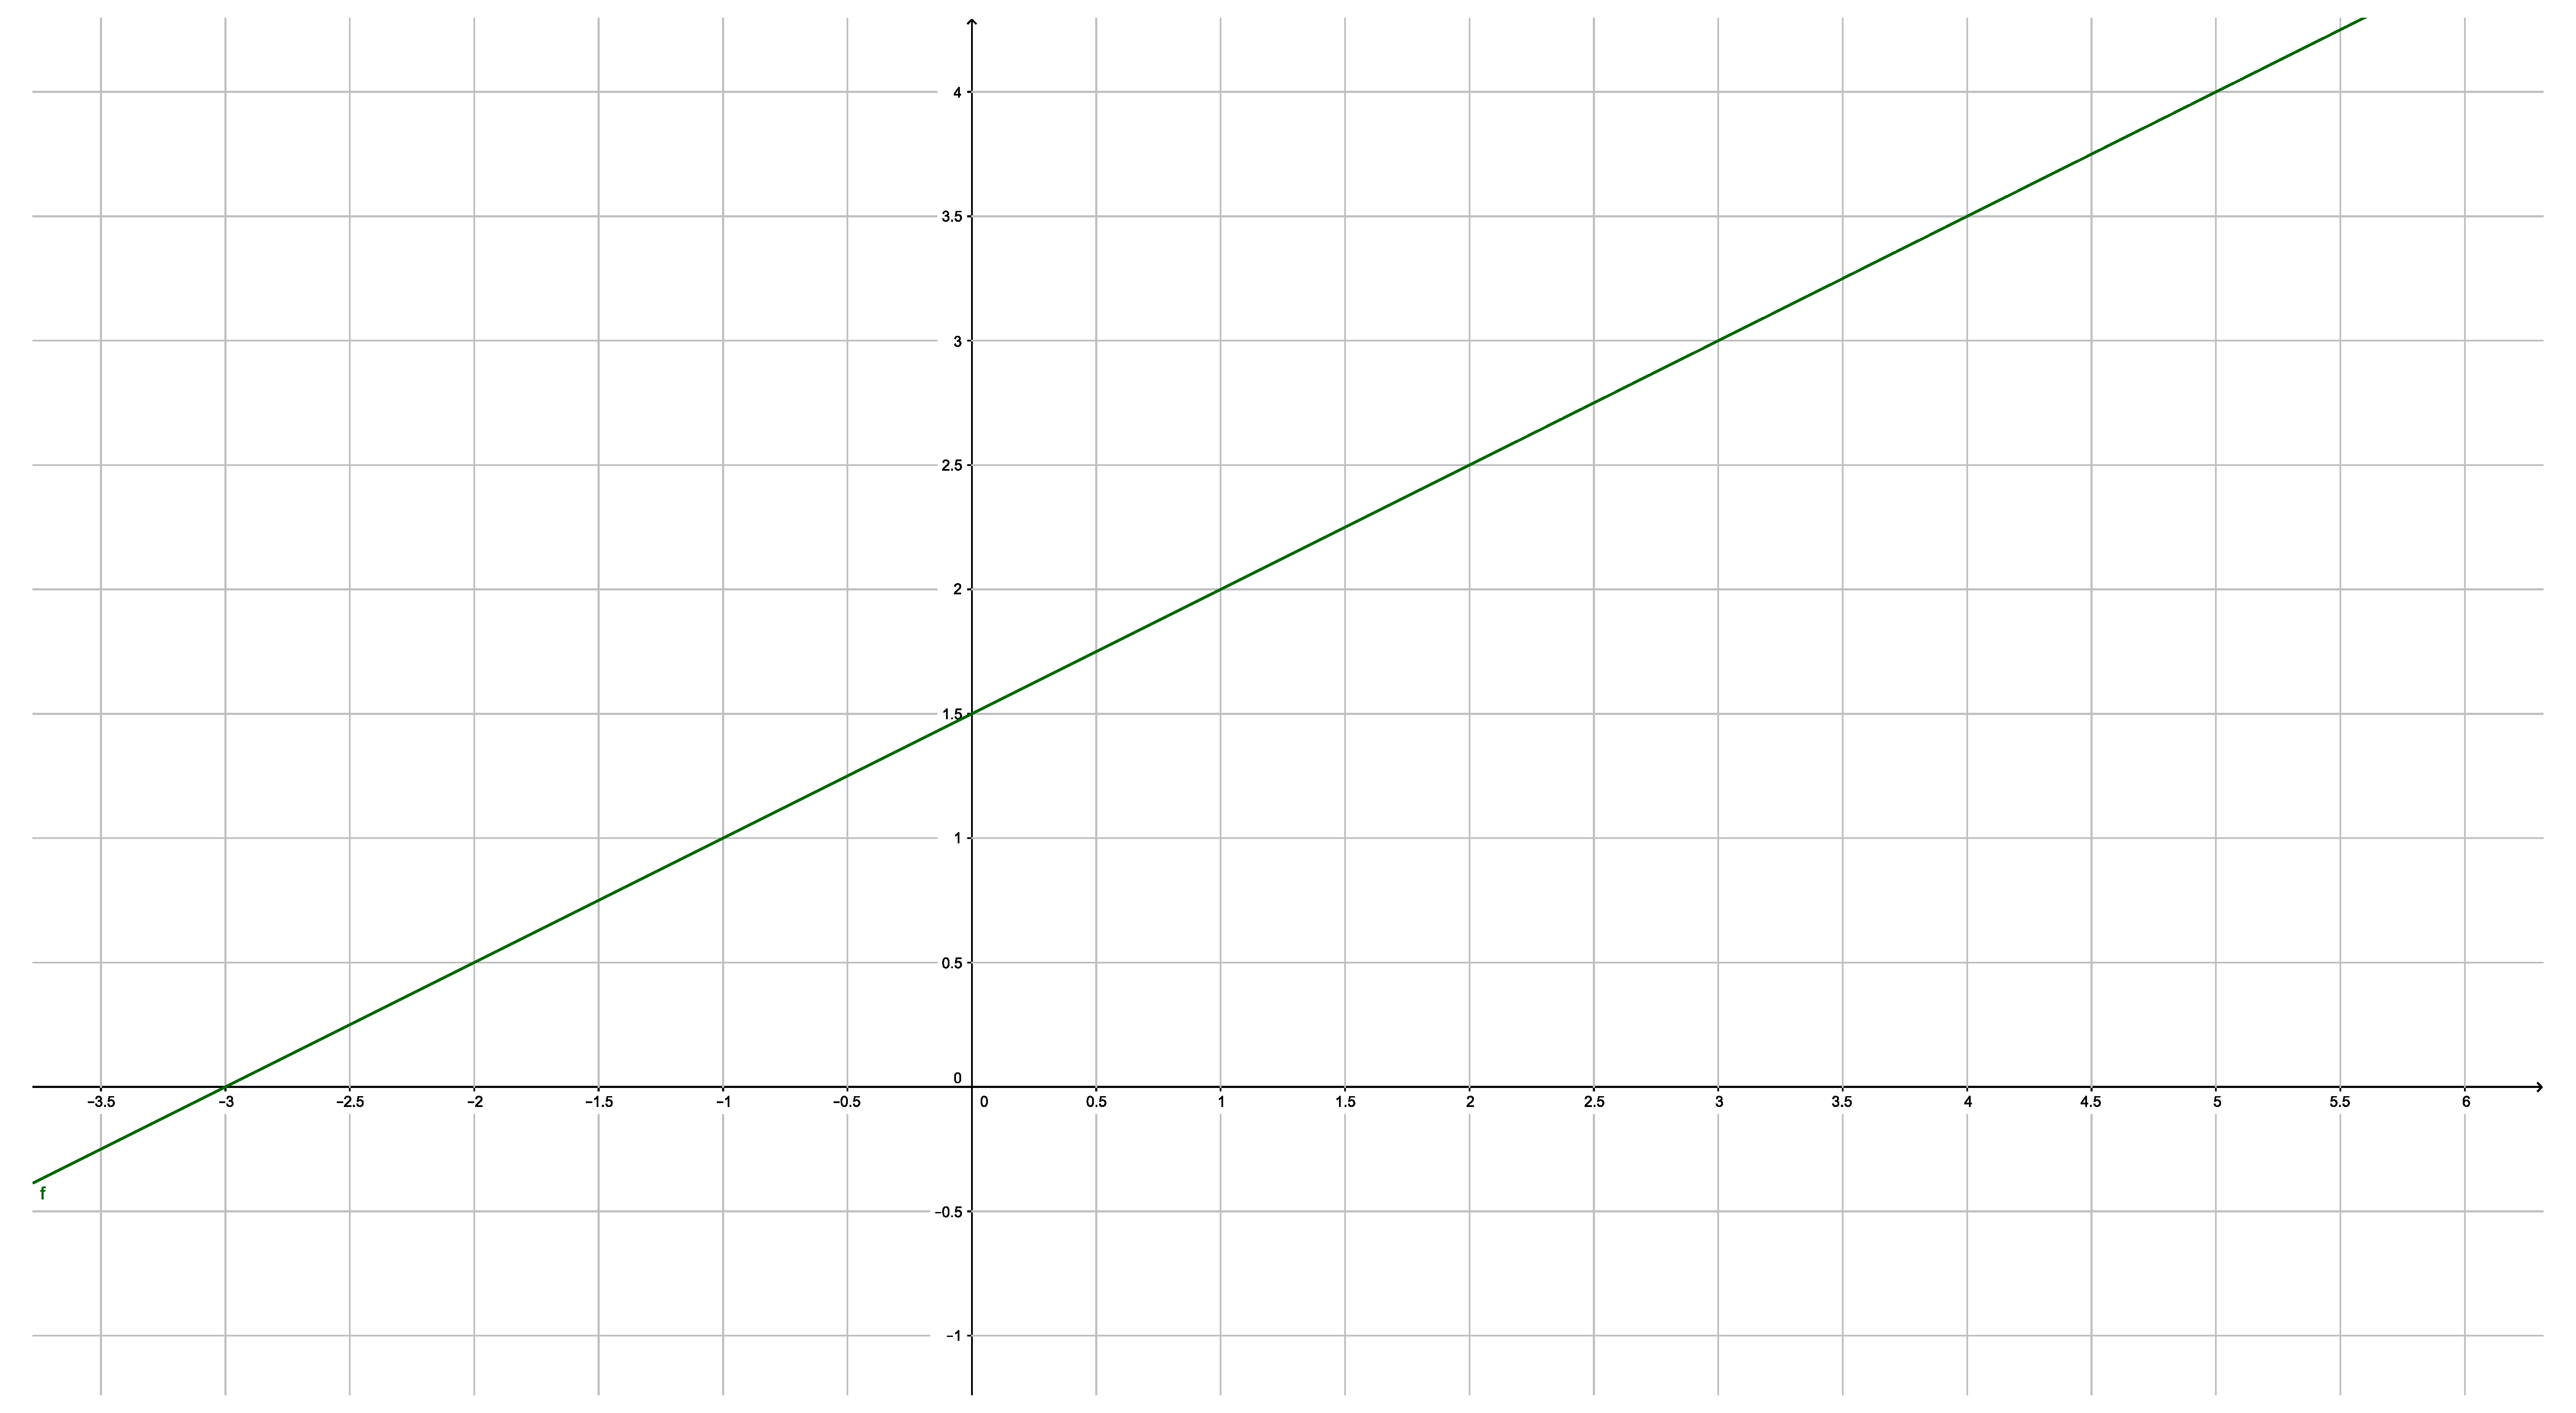
\includegraphics[width=200px, height=200px]{lineare.pdf}
			\captionsetup{labelformat=empty}
			\caption{\label{fig:blue_rectangle} $f(x)=0,5x+1,5$}
		\end{figure}
	\end{minipage} \hfill
	\begin{minipage}{0.45\textwidth}

	Beispiel:
		\begin{alignat*}{4}
		m &=\frac{\Delta y}{\Delta x} = \frac{ y_{2}-y_{1} }{x_{2}-x_{1} } \\
		  &\leftrightarrows \frac{3,5 - 1,5}{4 - 0} = 0,5
		\end{alignat*}
	\end{minipage}
	\newpage
	\subsubsection{Schnittpunkt zweier linearer Funktionen}
		\begin{tabular}[t]{llr}
			Der \textbf{Schnittpunkt} $x$ zweier linearer Funktonen berechnet sich durch das Gleichsetzen\\ zweier lineare Funktionen:\\
			$f(x) = 0,5x+1,5$\\
			$g(x) = 1x+0,2$

		\end{tabular}

		\begin{minipage}{0.5\textwidth}
			\begin{figure}[H]
				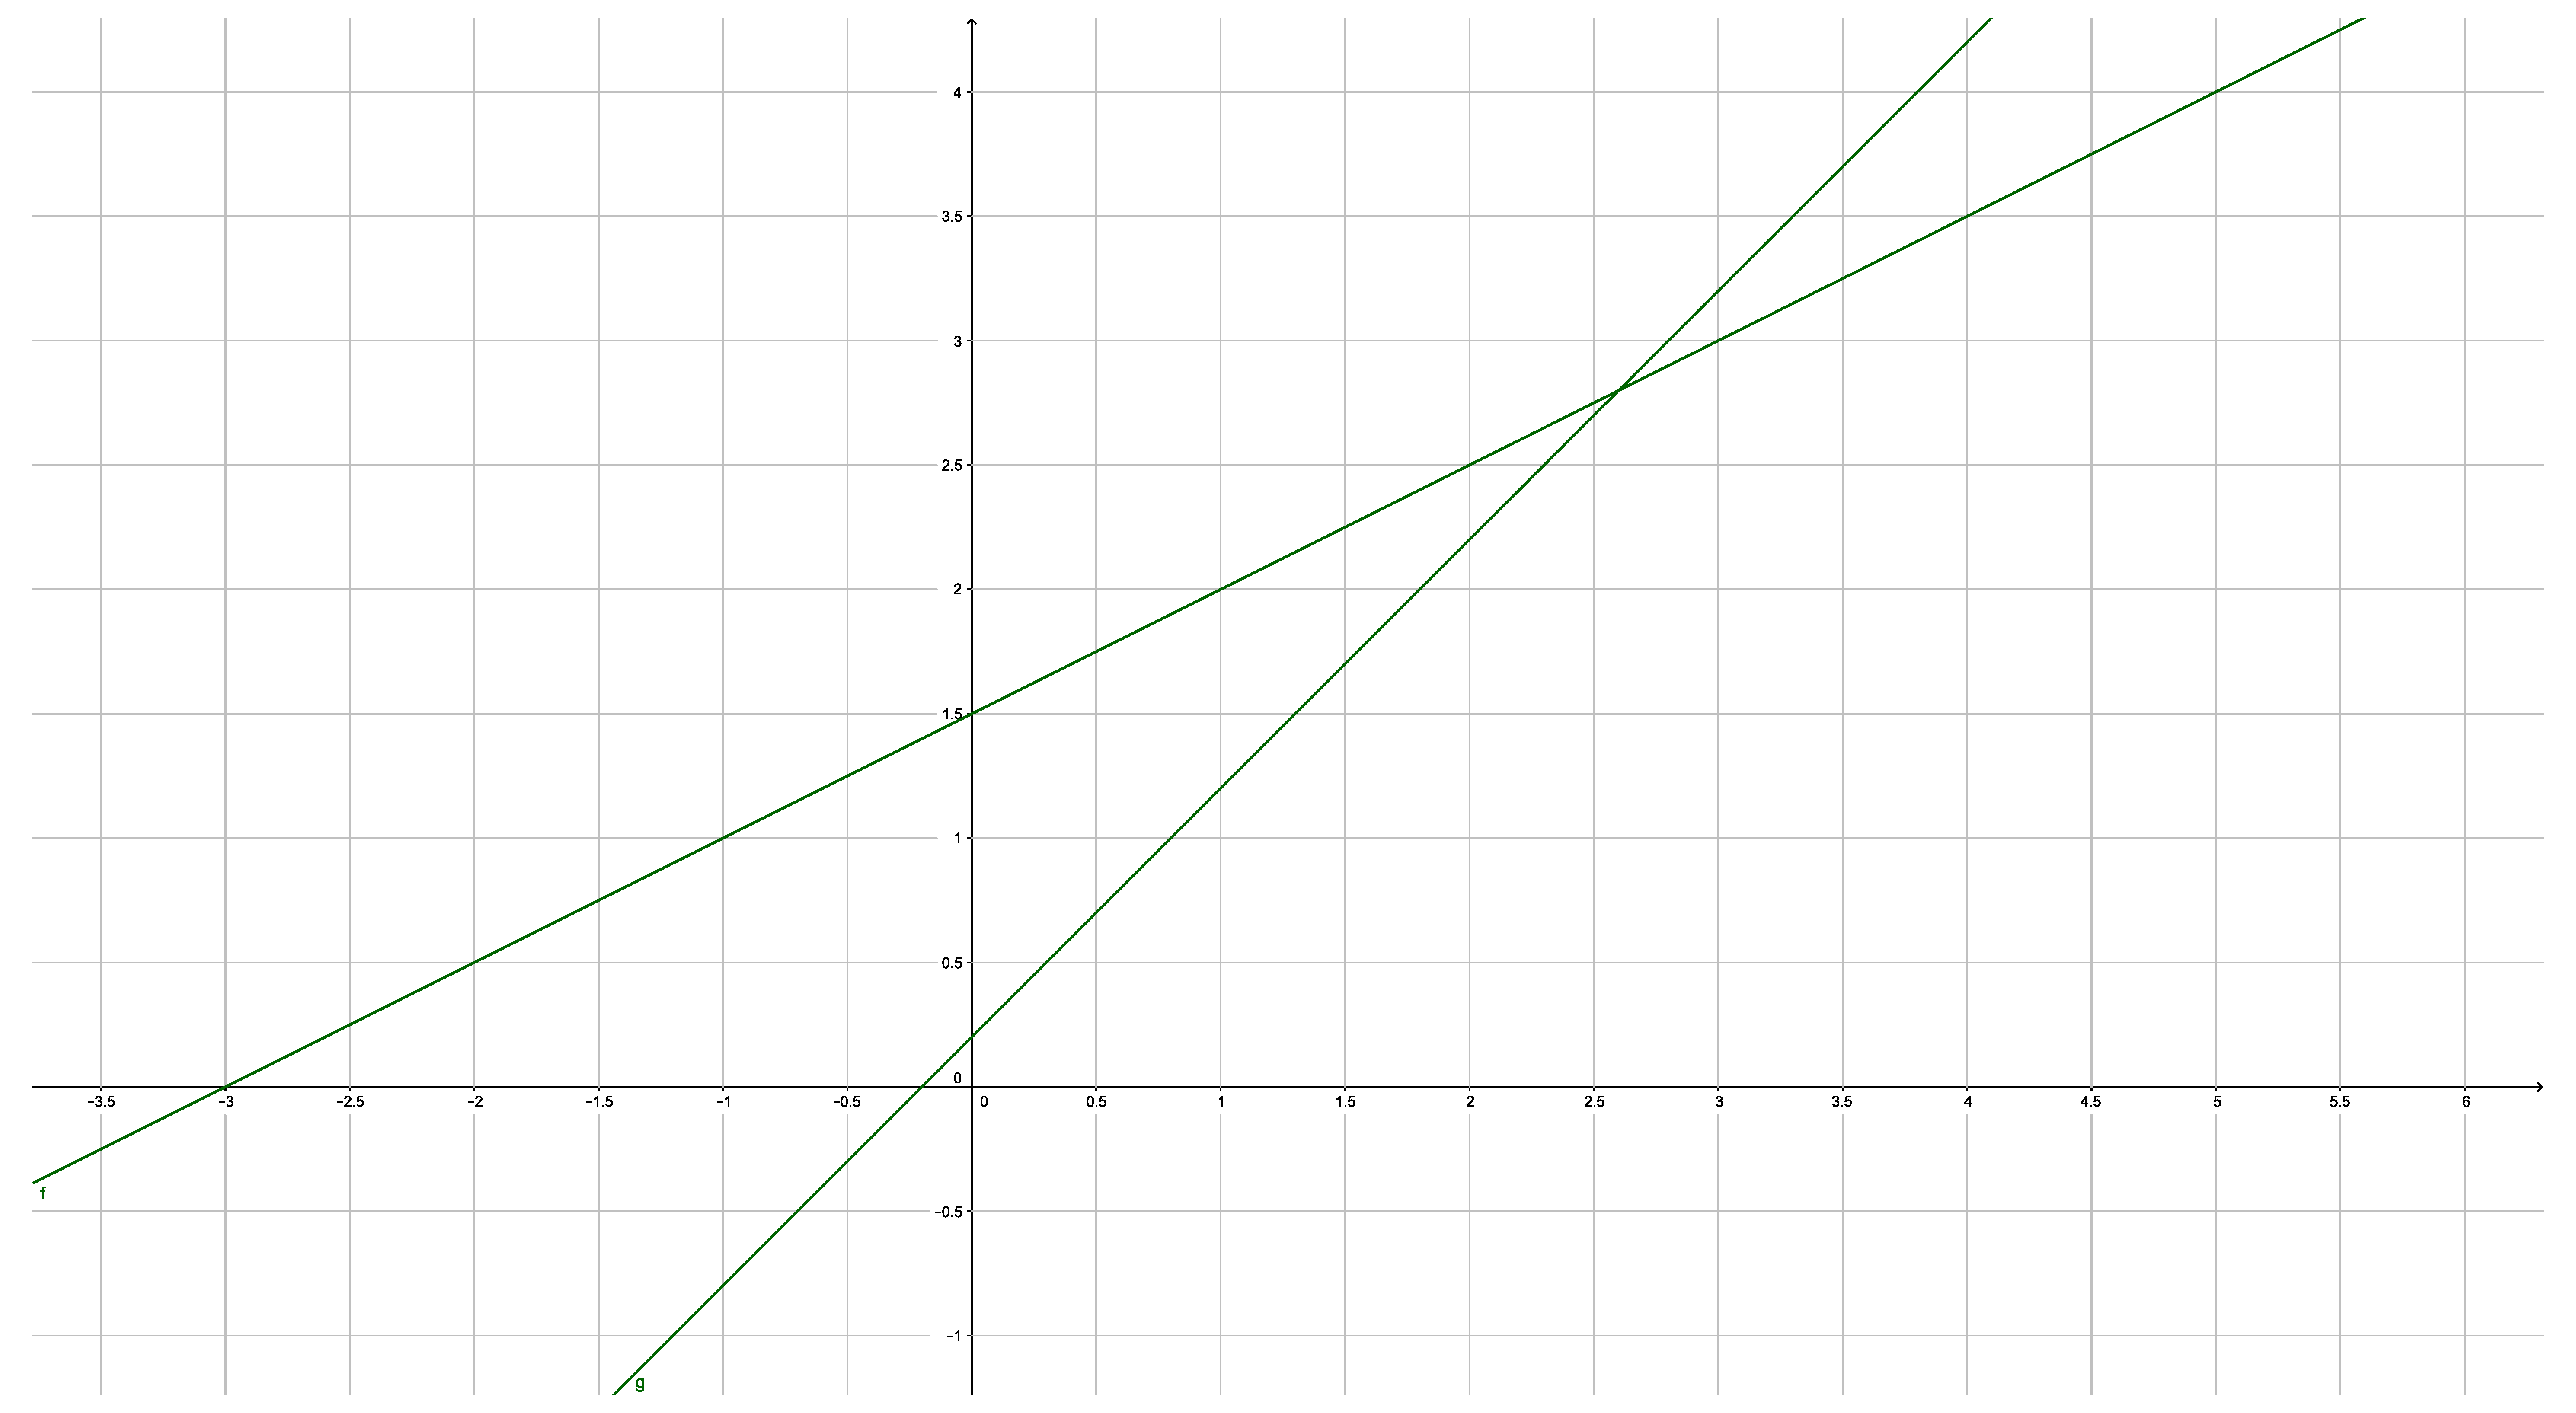
\includegraphics[width=200px, height=200px]{lineare2.pdf}
					\captionsetup{labelformat=empty}
				\caption{  }

			\end{figure}
		\end{minipage} \hfill
		\begin{minipage}{0.45\textwidth}
				Beispiel:
			\begin{alignat*}{4}
			0,5x+1,5 &= 1 && x +0,2 && |-0,5x \\
			1,5 	 &= 0,5 && x+0,2 && |-0,2\\
			1,3 	 &= 0,5 && x &&|*2 \\
			2,6		 &=  && x
			\end{alignat*}
				Jetzt kann das Ergebnis\\($x=2,6$) in die Gleichungen eingesetzt werden um das Ergebnis zu ueberpruefen.\\
				$f(2,6) = 2,8$\\
				$g(2,6) = 2,8$\\
				Da die beiden Werte gleich sind heisst das, dass die Rechnung korrekt ist.


		\end{minipage}
	\newpage
	\subsection{Quadratische Funktionen}
	\begin{tabular}[t]{llr}
			Eine quadratische Funktionen ist eine Funktion der Form $ f(x)= ax^{2}+bx+c$ in der Normal\\ -und $f(x) = a(x-x_s)^{2}+y_s$ in der Scheitelpunktform.
		\end{tabular}\\
		\begin{tabular}[t]{llr}
		\begin{minipage}{0.5\textwidth}
			\begin{figure}[H]
				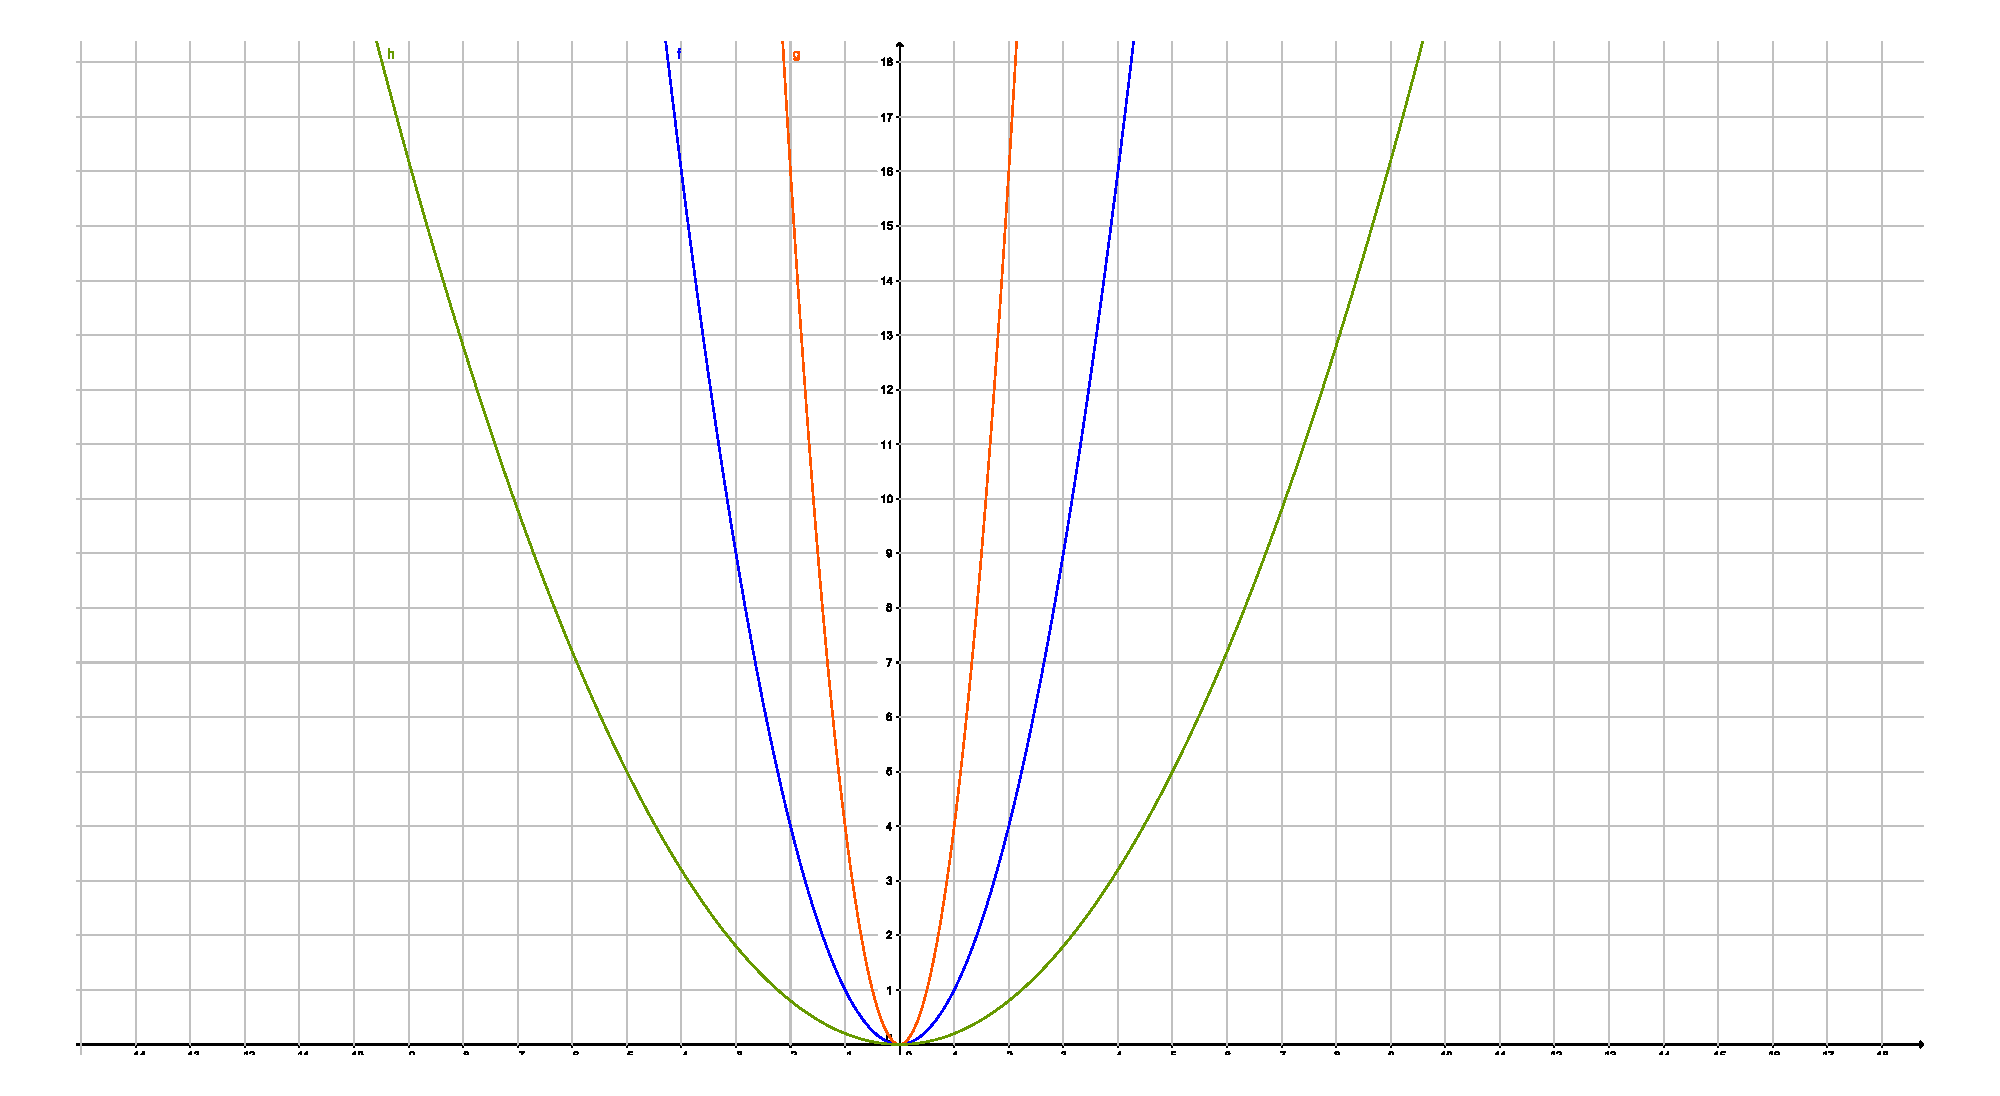
\includegraphics[width=200px, height=200px]{quadr-B.pdf}

				\captionsetup{labelformat=empty}
				\centering
				\caption{Gestreckte Parabel:\\  $h(x) =0,2x^{2}+0x+0; \hspace{0,3 cm} 0,2(x-0)^2+0$ }
				\vspace{-0,3 cm}
				\caption{Normale Parabel:\\ $f(x) =1x^2+0x+0; \hspace{0,3 cm}1(x-0)^2+0  $}
				\vspace{-0,3 cm}
				\caption{Gespreizte Parabel\\ $g(x)=4x^2+0x+0; \hspace{0,3 cm}4(x-0)^2+0 $}

			\end{figure}
		\end{minipage}
		\end{tabular}
		\begin{minipage}[t]{0.5\textwidth}
			\vspace{-3.8 cm}

		\end{minipage}

	\subsubsection{Eigenschaften einer quadratischen Funktionen}
	Die Verschiedenen Koeffinzienten einer quadratichen Funktion, haben verchiedene Auswirkungen auf das Aussehen einer
	quadratischen Funktion.\\
	\\ \textbf{Normalform:}\\
	Der \textbf{Koeffizient $a$} gibt sowohl die Oeffnungsrichtung als auch die Steigung einer Parabel wieder, ist $a < 0$ ist die Parabel nach unten geoeffnet, ist $a > 0$ ist sie nach oben geoeffnet. Ist $a = 0$ ensteht eine lineare Funktion.\texttt{}\\
	Ueber die Steigung kann man folgene Aussagen treffen: Ist $a > 1$ ist die Parabel gestreckt, ist $a<1$ ist sie gespreitzt, $a=1$ stellt die Normalparabel da.
	\\\\Der \textbf{Koeffinzienten $b$} gibt die Steigung der Parabel im Schnittpunkt mit der Ordinate an, zusaetlich laesst sich am Vorzeichen ablesen
	ob die Parabel die Ordinate, mit dem fallenden Ast der Parbel geschnitten wird oder mit dem Steigenden.
	Ist $b < 0$, scheidet der fallende Ast die Ordinate, sonst der Andere.
	Eine Veraenderung des Koeffinzienten $b$ bewirkt eine Verschiebung sowohl in x- als auch in y-Richtung. Wird $b$ um eins eroeht, dann wird der Graph um $\frac{1}{2a}$ Einheiten nach links und $\frac{2b+1}{4a}$ nach unten verschoben. Wird b um eins verringert, wird der Graph dagegen um $\frac{1}{2a}$ Einheiten nach rechts und $\frac{2b-1}{4a}$ nach oben verschoben.



	\hspace{-1.5 cm}
	Der \textbf{Koeffizient $c$} bestimmt wie die Funktion auf der Ordinatenachse verschoben ist.


	\subsubsection{Umwandlung der Normalform in die Scheitelpunktform}

		Es sei $f(x)=2x^2+2x+5$, um diese Funktion in die Scheitelpunktform zu ueberfuehren\\ muessen folgende Schritte vollzogen werden.

		\begin{alignat*}{4}
		%%%%%%%%%%%%%%%%%%%%%%%%%%%%%%%%%%%%%%%%%%%%%%%%%%%%
		%Nochmal allgemeingueltig |SP \hspace{0.1 cm} der Funktion, Werte einzs\\
		%%%%%%%%%%%%%%%%%%%%%%%%%%%%%%%%%%%%%%%%%%%%%%%%%%%%5%%
		 f(x) 						&=  (ax^{2}    	     + && bx) 										 	   							  &&+c     && \hspace{0.3 cm}|a \hspace{0.1 cm} ausklammern \\
									&= a\bigg( x^{2} 	     + && \frac{b}{a}x \bigg) 						 		   	   							  && +c    && \hspace{0.3 cm}|q.E. \\
									&=  a \bigg[ x^{2}   + && 2\frac{b}{2a}x + \bigg(\frac{b}{2a}\bigg)^2 - \bigg(\frac{b}{2a}\bigg)^2 \bigg]&& +c    && \hspace{0.3 cm}|bin. Form\hspace{0.12 cm} rueckwaerts\\
									&=  a \bigg[\bigg( x + && \frac{b}{2a} \bigg)^{2}  - \bigg(\frac{b}{2a}\bigg)^2 \bigg]				  && +c    && \hspace{0.3 cm}|Klammer\hspace{0.1 cm} aufloesen\\
									&=  a \bigg( x       + && \frac{b}{2a} \bigg)^{2}  - \frac{ab^{2}}{4a^{2}} 							  && +c    && \hspace{0.3 cm}|a \hspace{0.1 cm} kuerzen \\ %%WIE GEHT DAS
									&=  a \bigg( x       + && \frac{b}{2a} \bigg)^{2}  +\bigg( c - \frac{b^{2}}{4a}\bigg) 				  &&       && \hspace{0.3 cm} |SPF \hspace{0.1 cm} der Funktion \\
		\end{alignat*}
		\hspace{-0.1 cm}
		Hier kann man nun den Scheitelpunkt ablesen: \\

		S =   $\bigg( -\frac{b}{2a}  | c - \frac{b^{2}}{4a}\bigg)$ =  $\bigg( -0,5  | 4,5\bigg)$
		\subsubsection{Schnittpunkt zweier quadratischer Funktionen}
		$f(x)=5x^2-10x+2$\\
		$g(x)=x^2+2x+0$

		\begin{align*}
			5x^2-10x+2 &= x^2+2x+0 & 	|&-2x\\
			5x^2-12x+2 &= x^2 & 		|&-x^2\\
			4x^2-12x+2 &= 0   & 		|&:4\\
			x^2-3x+0.5 &= 0
		\end{align*}
			Nun kann die Gleichung mit der P-Q-Formel geloest werden.
		\newpage
		\subsection{Funtionen mit dem Grad $> 2$}
		%\subsubsection{Substitution}
		%\subsubsection{Polynomdivision}
		\subsection{Trigonometrische Funktionen}
		Trigonmetrische Funktionen sind Funktionen der Form $a*<trig>(b*x+c)+d$, wobei $<trig>$ fuer einen Ausdruck wie die Sinus- oder Kosinusfunktion stehen kann z.B. ist $a*sin(x+5)$ eine trigonometrische Funktion.
		\subsubsection{Eigenschaften Trigonometrische Fuktionen\\}
		\textbf{Funktionen der Form $a*<trig>(x)$\\}
		Der Parameter \textbf{a} bestimmt die Auslenkung in Ordinatenrichtung, d.h. die Funktionswerte einer trigonometrischen Fuktion gehen von $-a$ bis  $a$.\\\\
		\textbf{Funktionen der Form $a*<trig>(x)+d$\\}
		Der Parameter \textbf{d} bestimmt die Verschiebung in Ordinatenrichtung d.h. die Funktionswerte gehen von $-a$ bis $a$ aber um $d$ verschoben.\\\\
		\textbf{Funktionen der Form $a*<trig>(b*x)+d$\\}
		Der Parameter \textbf{b} bestimmt die Periodizität der Funktion d.h. $f(x)=sin(x)$ hat eine Periode von $0$ bis $2\pi$ $g(x)=sin(2x)$ von $0$ bis $\pi$, die anderen Parameter haben keinen Einfluss auf die Peridizitaet.\\\\
		\textbf{Funktionen der Form $a*<trig>(c+b*x)+d$\\}
		Der Parameter \textbf{c} bestimmt die Verschiebung der Funktion auf der Abzisse z.B. ist die Funktion $f(x)=sin(0.5+x)$
		um $0.5\pi$ nach links verschoben

		\subsection{Tangente und Normale}
		\pagebreak
		\subsection{Exponentialfunktionen}
		\subsubsection{Natuerliche Expoentialfunktion}
		Als natuerliche Exponentialfunktion bezeichnet man Variationen der Funtion $f(x)=e^x$.
		\paragraph{Eigenschaften der Natuerlichen Exponentialfunktion}
		\hspace{0 cm} \\ \noindent \\
		\begin{minipage}{0.3\textwidth}
		\begin{figure}[H]
		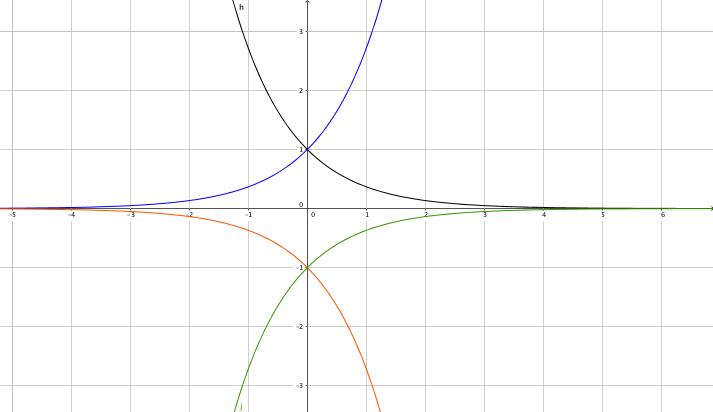
\includegraphics[width=300px, height=200px]{E_1.png}
			\captionsetup{labelformat=empty}
				\centering
				\caption{$e^x$}
				\vspace{-0,3 cm}
				\caption{$-e^x$}
				\vspace{-0,3 cm}
				\caption{$e^{-x}$}
				\vspace{-0,3 cm}
				\caption{$-e^{-x}$}
		\end{figure}
		\end{minipage} \hfill
		\begin{minipage}{0.5\textwidth}
		\end{minipage}\\\\
		\begin{minipage}{0.3\textwidth}
		\begin{figure}[H]
		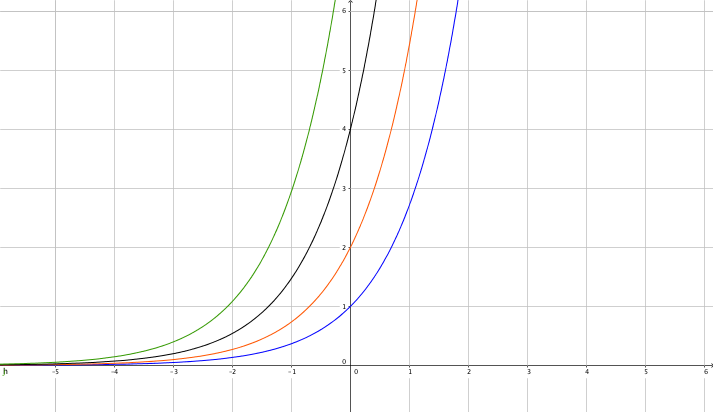
\includegraphics[width=300px, height=200px]{E_2.png}
			\captionsetup{labelformat=empty}
				\centering
				\caption{$e^x$}
				\vspace{-0,3 cm}
				\caption{$2e^x$}
				\vspace{-0,3 cm}
				\caption{$4e^{x}$}
				\vspace{-0,3 cm}
				\caption{$8e^{x}$}
		\end{figure}
		\end{minipage} \hfill
		\\\\
		\begin{minipage}{0.3\textwidth}
		\begin{figure}[H]
		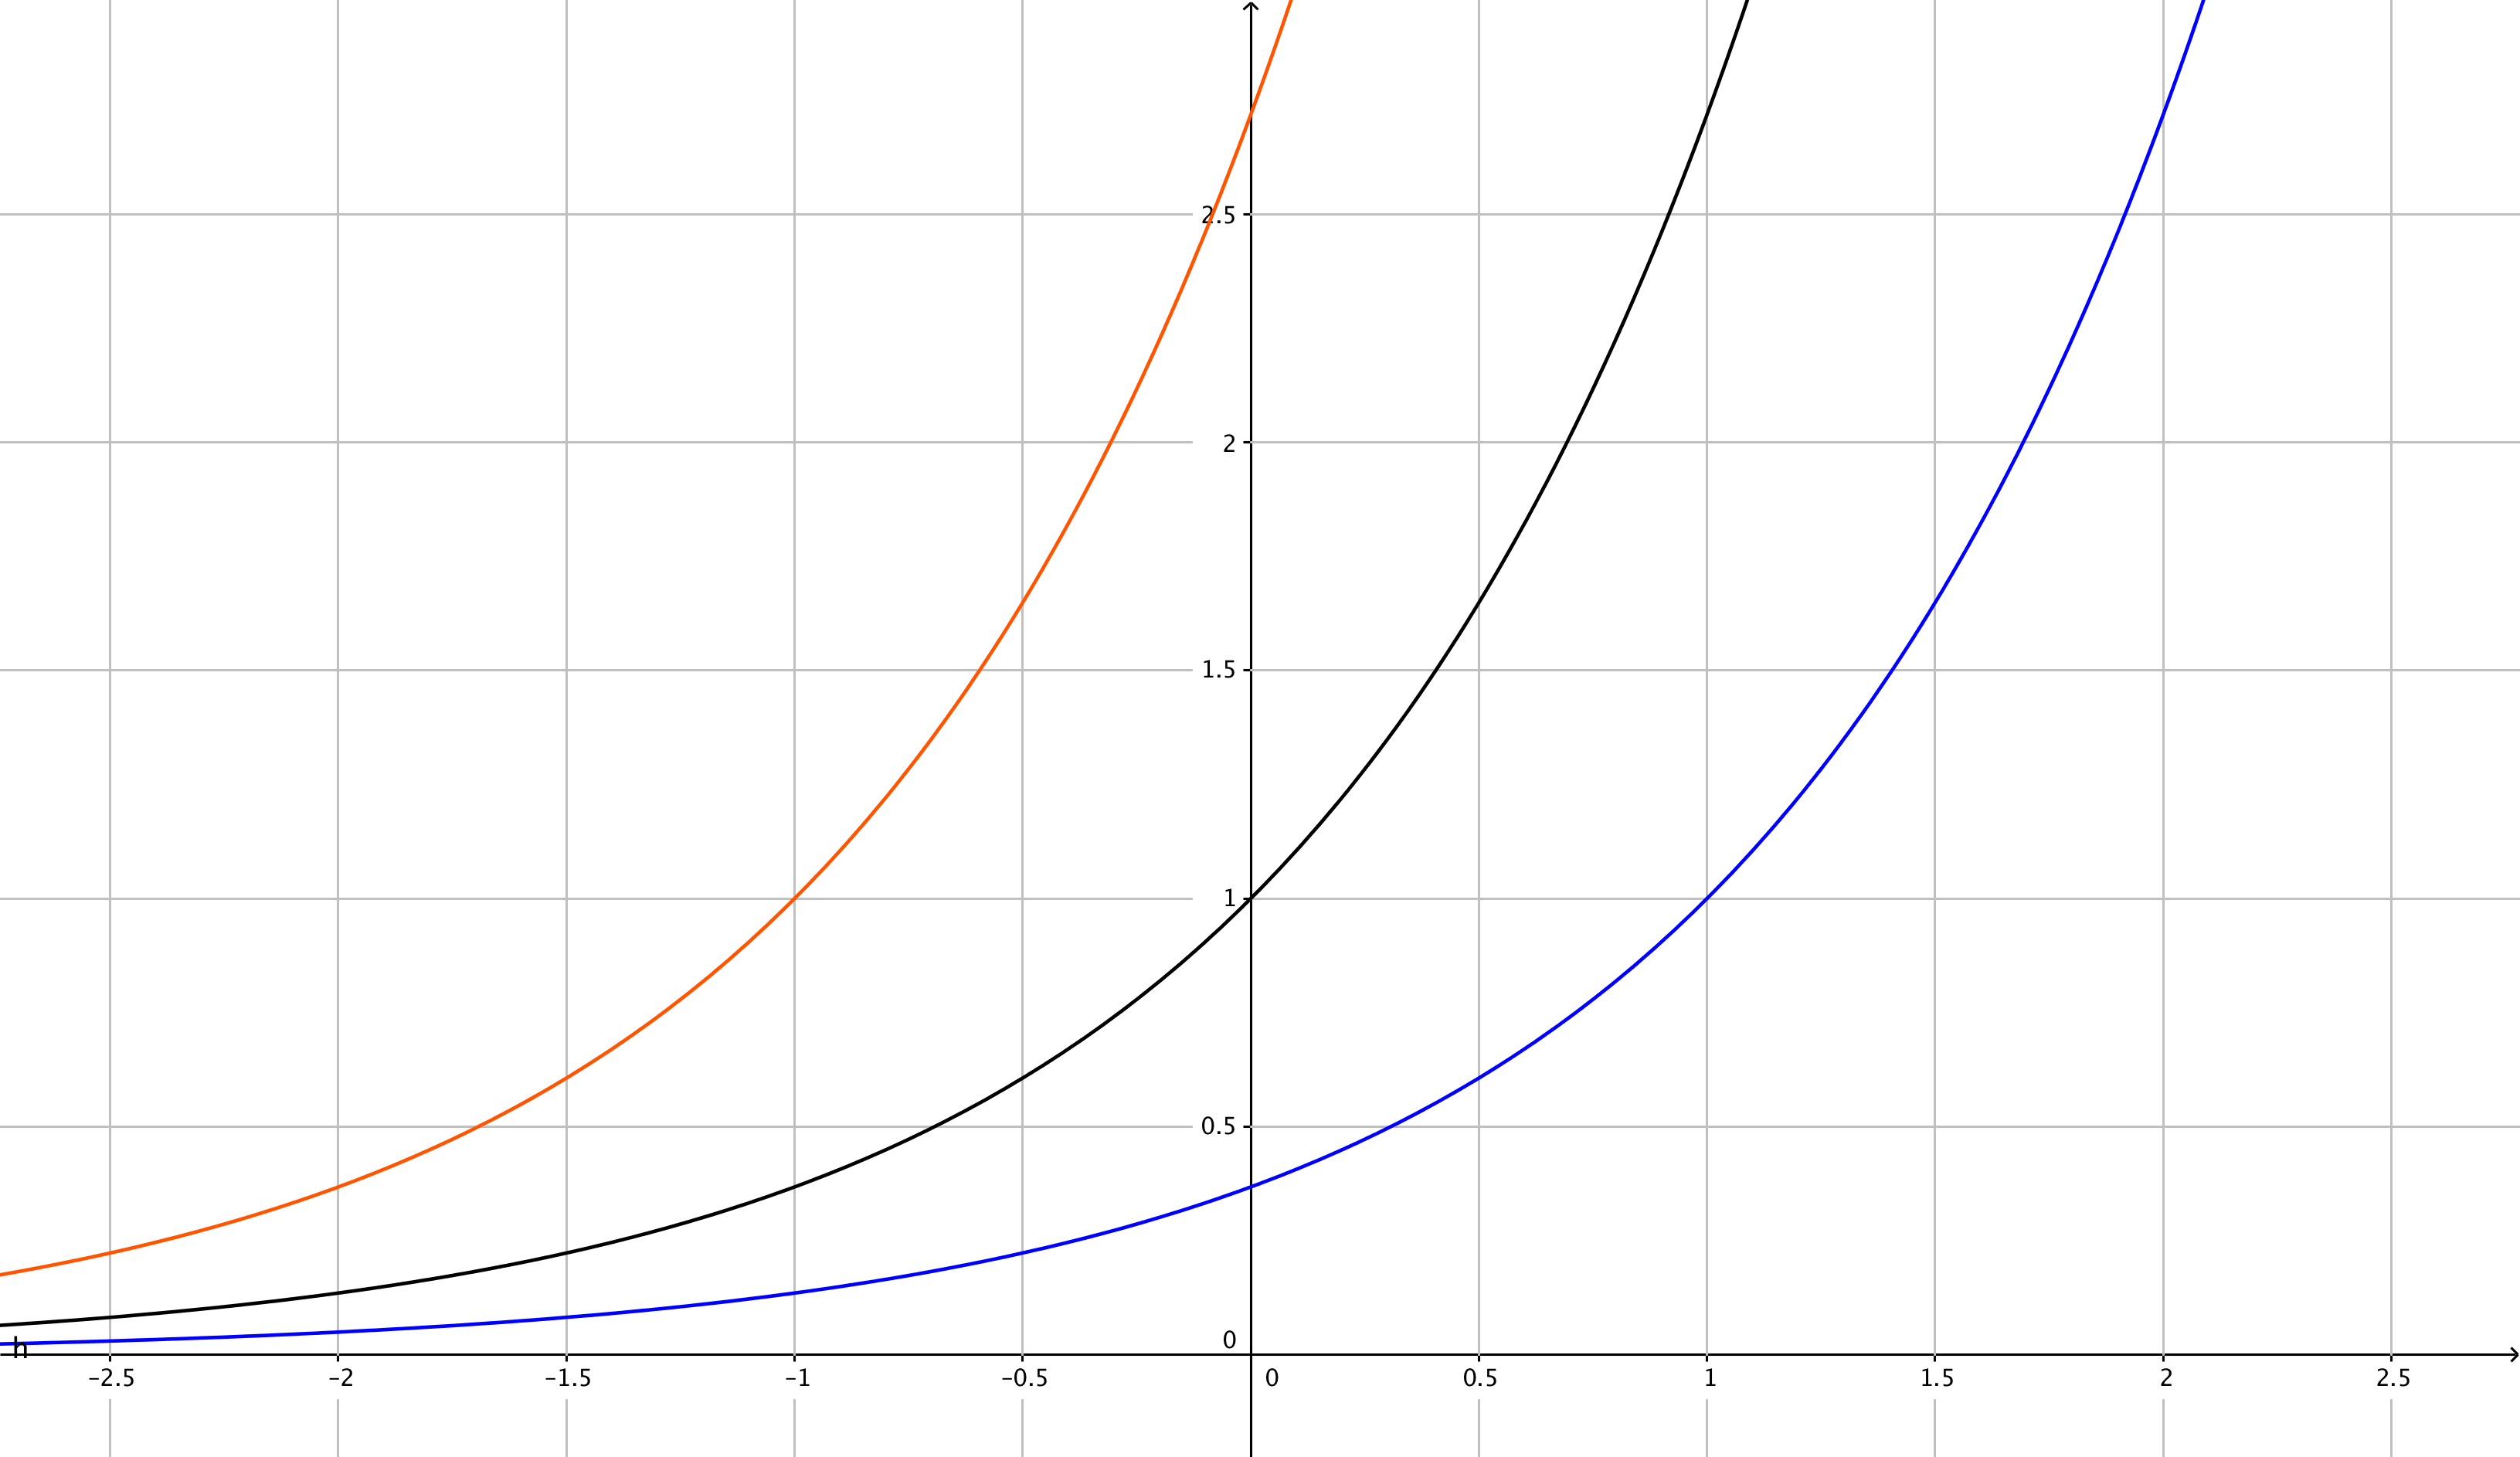
\includegraphics[width=300px, height=200px]{E_3.png}
			\captionsetup{labelformat=empty}
				\centering
				\caption{$e^{x-1}$}
				\vspace{-0,3 cm}
				\caption{$e^{x+1}$}
				\vspace{-0,3 cm}
				\caption{$e^{x}$}
		\end{figure}
		\end{minipage} \hfill
		\\\\
		\begin{minipage}{0.3\textwidth}
		\begin{figure}[H]
		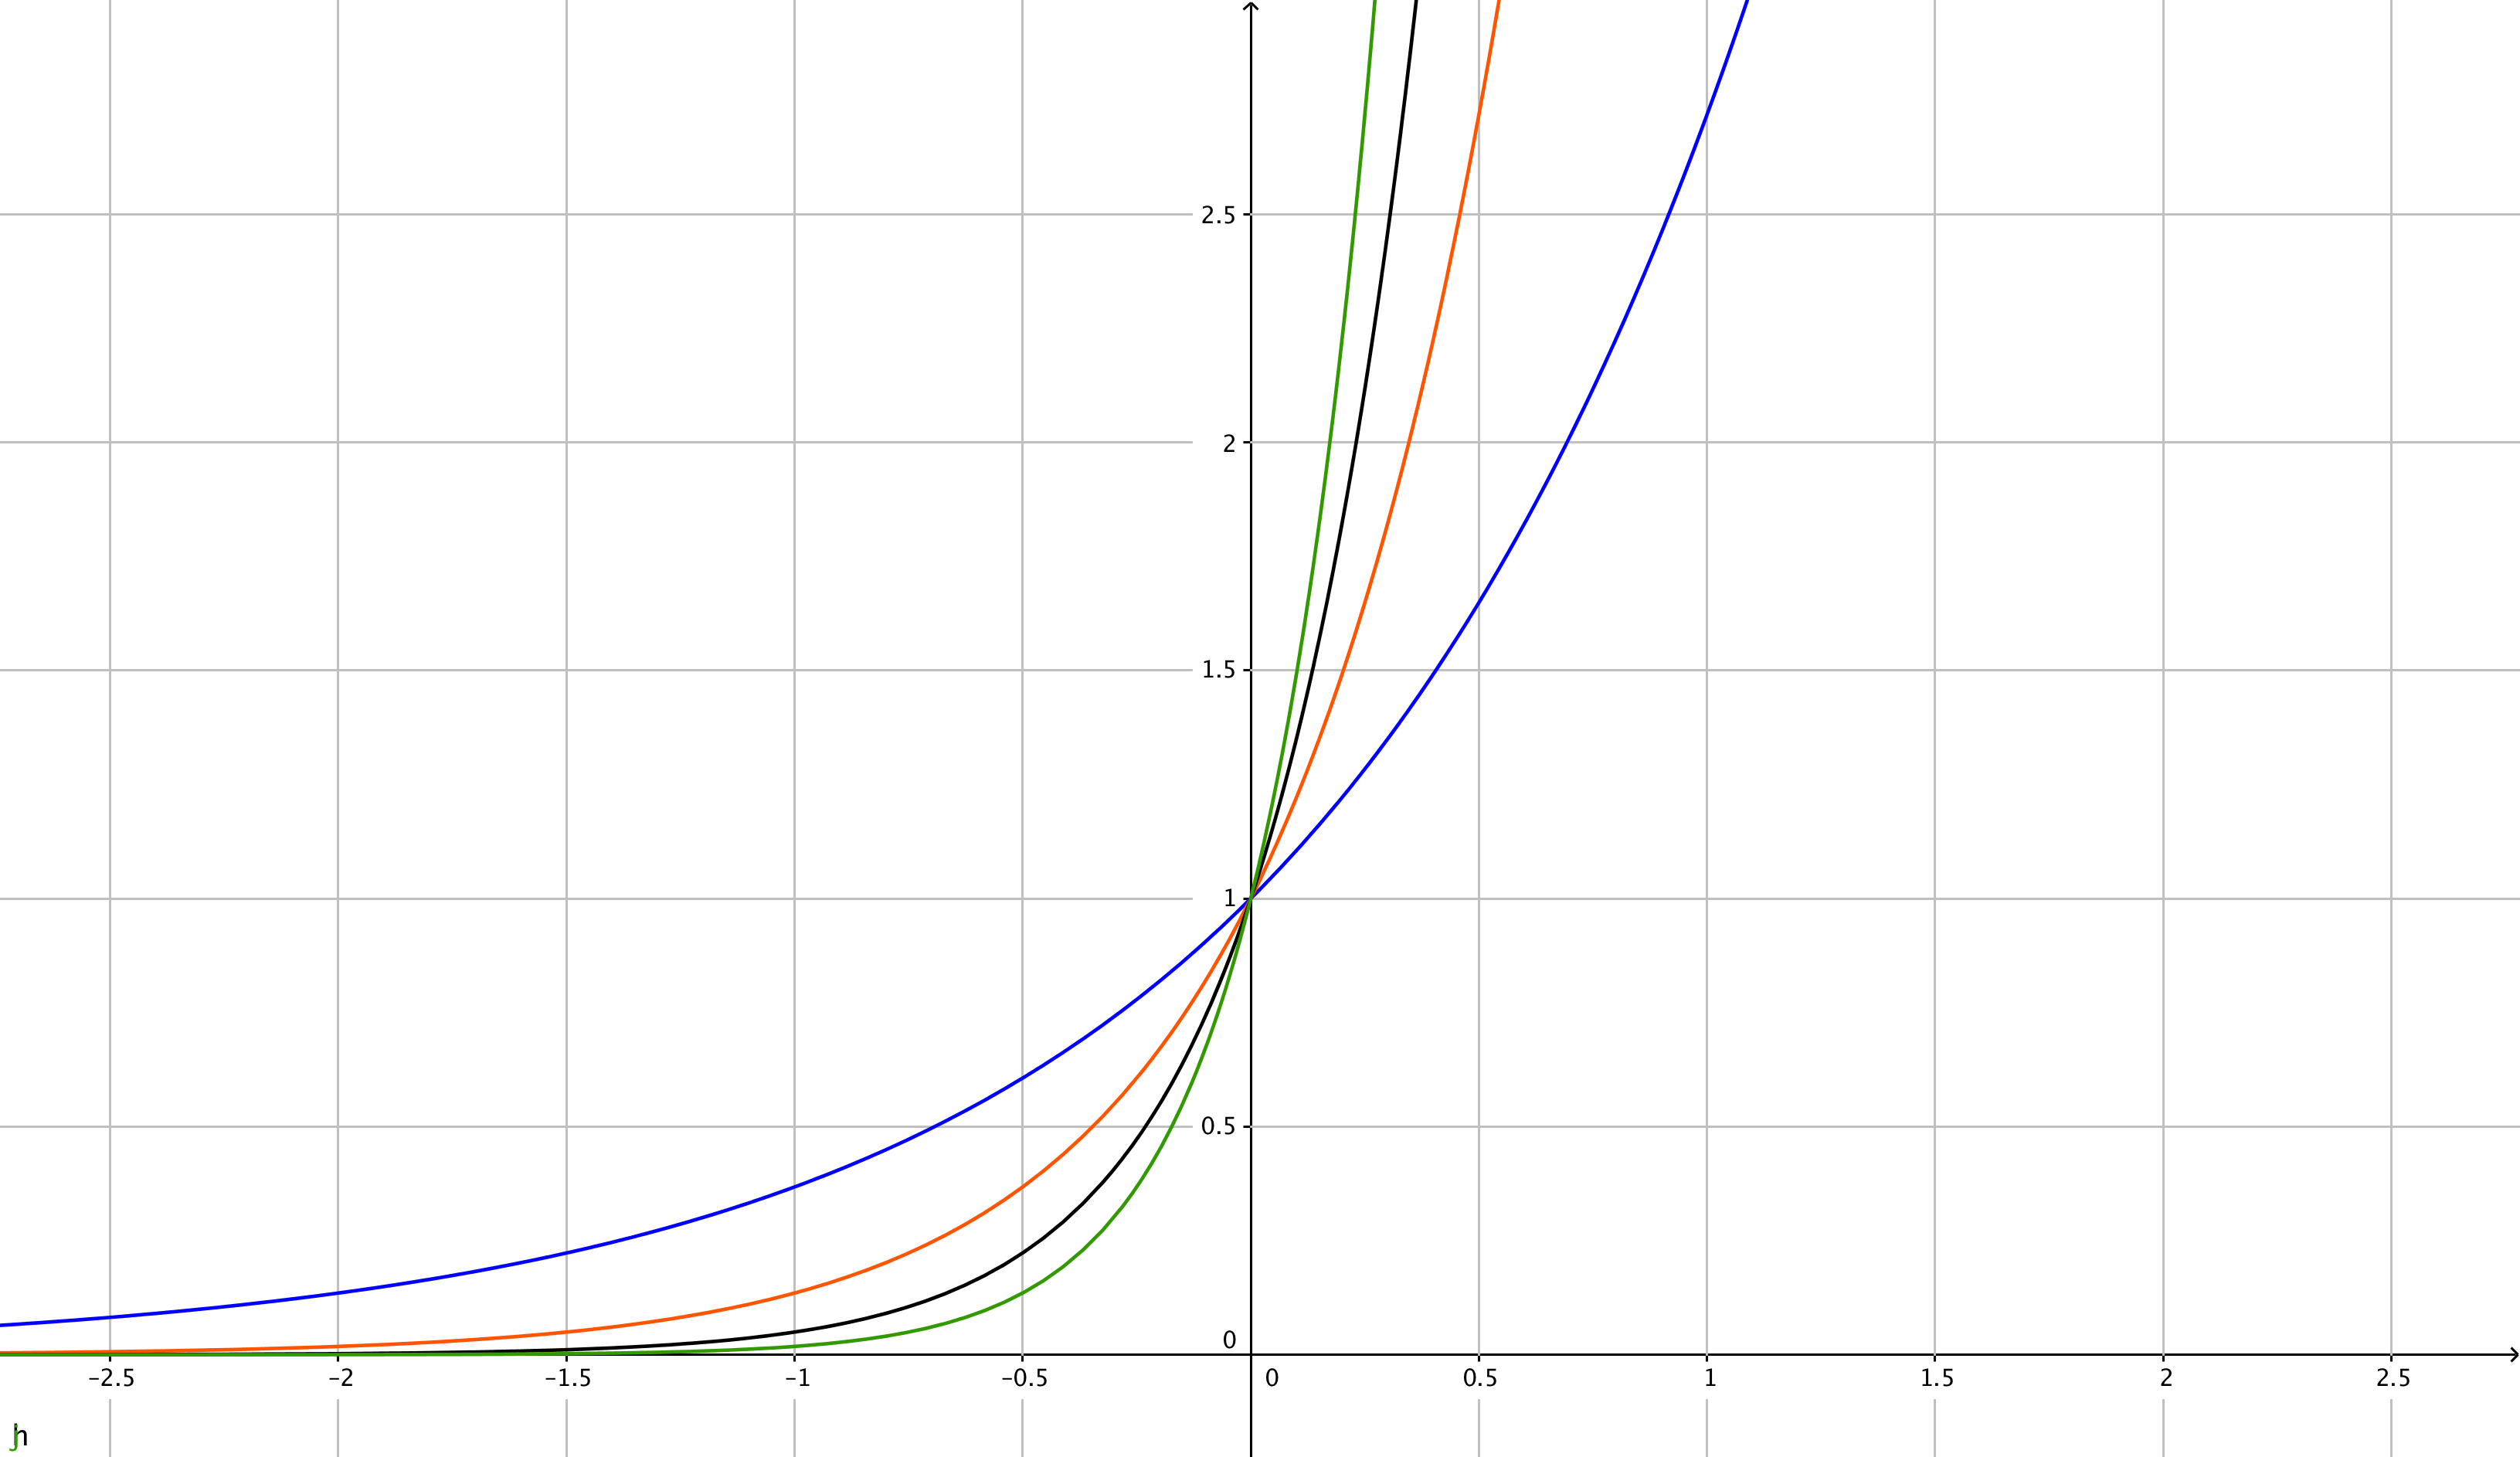
\includegraphics[width=300px, height=200px]{E_4.png}
			\captionsetup{labelformat=empty}
				\centering
				\caption{$e^{x}$}
				\vspace{-0,3 cm}
				\caption{$e^{2x}$}
				\vspace{-0,3 cm}
				\caption{$e^{3x}$}
				\vspace{-0,3 cm}
				\caption{$e^{3x}$}
		\end{figure}
		\end{minipage} \hfill

		%\subsection{Umkehrfunktion}
		\subsection{Funktionenscharen}
		%\subsection{Herleitung}
		%\subsubsection{Trigonometrische Funktionen}
		%\subsubsection{Quadratische Ergaenzung}
		%\subsubsection{P-Q-Formel}
		%\subsubsection{Polynomdivision}
		%\subsubsection{Horner Schema}
	\newpage
	\section{Differentialrechnung}
	\subsection{Visualisierung}


	\begin{minipage}{0.3\textwidth}
	\begin{figure}[H]
	\includegraphics[width=300px, height=200px]{a.eps}
	%\includegraphics[width=300px, height=200px]{Ableitung_1.png}
	\caption{}
	\end{figure}
	\end{minipage} \hfill
	\begin{minipage}{0.5\textwidth}

	Hier zu sehen ist der Graph $f(x)$, mit seinen Ableitungen $f'(x)$ und $f''(x)$.
	Hier kann man sehr gut erkennen wie die Nullstellen der 1. Ableitung $f'(x)$, genau an
	der Position liegen an der auch die Steigung von $f(x)$ gleich 0 ist.\\
	Schaut man sich nun die 2. Ableitung an, kann man erkennen das sich Nullstelle der 2. Ableitung an der Stelle befinden wo $f(x)$ einen Wendepunkt hat.

	\end{minipage}




%	\end{tabular}
	\subsection{Bedeutung der 1. Ableitung}

	Die 1. Ableitung gibt die Steigung der Originalfunktion wieder, d.h wenn die 1. Ableitung 0 ist \\hat die Originalfunktion an diesem Punkt eine
	Steigung von 0 und damit einen moeglichen Extrempunkt.

	\subsection{Bedeutung der 2. Ableitung}
	Die 2. Ableitung gibt die Steigung der 1. Ableitung wieder, d.h wenn die 2. Ableitung 0 ist \\hat die 1. Ableitung an diesem Punkt eine
	Steigung von 0. und damit hat die Originalfunktion an diesem Punkt meisstens einen Steigunswechsel.
	\subsection{Kurzform des Ableitens}

	Das Ableiten besitzt eine Kurzform, ohne jedes mal den Limes benutzen zu muessen, dabei muss man die Ableitungsregeln sowie die Tatsache dass ein konstanten Summand beim Ableiten wegfaellt beachten(Summenregel).
\\	Beispiel:\\
		\begin{align*}
	f(x)  &= 5x^2+3x^1-5x^0\\
	f'(x)  &= 2*5x^{2-1}+1*3x^{1-1} = 10x^1+3x^0\\
	\end{align*}
	In Worte gefasst bedeutet das, dass der Originalexponent vor den Koeffizenten gezogen und mit diesem multipliziert wird, danach wird der Exponent um 1 dekrementiert.

	\subsection{Ableitungsregeln}
	\subsubsection{Summenregel}
	Summen von Funktionen werden getrennt abgeleitet. \\
	Beispiel: \\
		\begin{align*}
			f(x) &= 5x^2+8x  \\
			 f'(x)&= 10x+8
		\end{align*}
	\subsubsection{Faktorregel}
	Konstante Faktoren bleiben beim Ableiten erhalten. \\
	Beispiel: \\ \begin{align*}
					f(x)&= 5*x^2 \\
					f'(x) &= 5*2x
				\end{align*}

	\subsubsection{Produktregel}
	\begin{align*}
		f(x)&=u(x)*v(x)\\
		f'(x)&=u'(x)*v(x)+u(x)*v'(x)
	\end{align*}

	%\begin{equation}
	%	f(x)=u(x)*v(x)\\
		% f'(x)=u'(x)*v(x)+u(x)*v'(x)
	% \end{equation}
	Beispiel: \\
	\begin{align*}
		f(x) &= 5x^2*8x-1  \\
		f'(x)&= 10x*8x+5x^2*8
	\end{align*}
	\subsubsection{Kettenregel}
	''Auessere mal innere Ableitung.''\\
	Ist eine Funktion das Ergebnis der Vekettung von 2 anderen Funktionen dann gilt:\\
	 \begin{align*}
		f(x)&=(u \circ v)(x)\\
		f'(x)&=u'(v(x))*v'(x)
	\end{align*}
	\\Beispiel:\\
		\begin{align*}
		f(x) &=e^{5x}\\
		f'(x)&=5e^{5x}
		\end{align*}

		\begin{align*}
		f(x)&=sin(5x)\\
		f'(x)&=5*cos(5x)
		\end{align*}

	\subsubsection{Quotientenregel}
		\begin{align*}
		f(x)&=\frac{u(x)}{v(x)}\\
		f'(x)&=\frac{u'(x)*v(x)-u(x)*v'(x)}{(v(x))^2}
		\end{align*}
		Beispiel: \\

	\subsection{Ableitung der $e$-Funktion}
	Die Ableitung der Funktion $f(x)=e^x$ ist $f'(x)=e^x$
	\\Beispiel:\\
	\begin{align*}
		f(x)&=5e^x\\
		f'(x)&=5e^x
	\end{align*}
	\subsubsection{Ableiten komplizierter $e$-Funktionen}
	Beim Ableiten der $e$-Funktion ist zu beachten, dass aufgrund der Position der Variable die \textbf{Kettenregel}
	beachtet werden muss.\\\\
	Beispiel
	\\\begin{align*}
	f(x)&=5e^{4x-2}\\
	f'(x) &=4*5e^{4x-2} \hspace{0.5cm}
	\end{align*}
	\subsection{Ableitung trigonometrischer Funktionen}
	\begin{align*}
	f(x) &= sin(x)\\
	f'(x) &= cos(x)\\
	f''(x) &= -sin(x)\\
	f'''(x) &= -cos(x)\\
	f''''(x) &= sin(x)
 	\end{align*}
 	\subsubsection{Ableitung komplizierter trigonometrischer Funktionen}
	%\subsection{Herleitungen}
	%\subsubsection{Herleitung der Ableitung mithilfe des Limes}
	%\subsubsection{Herleitung der Potenzregeln in  $\mathbb{N}$}
	%\subsubsection{Herleitung der Ableitung der $e$-Funktion in $\mathbb{N}$ mit Hilfe des Limes}
	%\subsubsection{Herleitung der Ableitung der Trigofunktion mithilfe des Limes}
	%\subsubsection{Herleitung der Ableitungsregeln}
	\pagebreak
	\section{Integralrechnung}
	\subsection{Unbestimmtes Integral}
	Unbestimte Integrale haben die Form,\\\\
	\begin{align*}
	\int f(x)=F(x)+C\\
	\end{align*}\\
	sie existieren auf Grund der Eingeschaft dass beim Ableiten Informationen verloren gehen.\\
	Beispiel\\
	\begin{align*}
	f(x) & =x^2+5\\
	f'(x) & =2x
	\end{align*}\\
	Wenn man nun $f'(x)$ integriert erhaellt man $F(x) =x^2$, $+5$ ist also verloren gegangen.
	Um dies darzustellen wird eine Integrationskonstante an $F(x)$ angehaengt, die korrekte Stammfunktion waere also $F(x)=x^2+C$.
	\subsection{Bestimmtes Integral}
	Um das bestimmte Integral einer Funktion zu berechnen muss, muss ein Wertepaar der Funktion gegeben sein, zum Beispiel
	das Wertepaar $(2;4,667)$ und die Stammfunktion $F(x)=\frac{1}{3}x^3+C$ oder ihre Ableitung.\\
	\begin{align*}
	F(x) & =\frac{1}{3}x^3+C\\
	4,667 &= \frac{1}{3}*8+C\\
	4,667 &= \frac{8}{3}+C\\
	2 & =C
	\end{align*}\\
	Die Funktion lautet also $F(x)=\frac{1}{3}*x^3+2$
	\subsection{Integrationsregeln}
	\subsubsection{Summenregel" der Integration}

	\begin{align*}
	h(x)=f(x)+g(x)=>H(x)= F(x)+ G(x)
	\end{align*}


	\subsubsection{Faktorregel}
	Konstante Faktoren bleiben beim Integrieren erhalten.
	\begin{align*}
	h(x) = r * f(x) => H(x)=r*F(x)
	\end{align*}
	\subsubsection{Kettenregel der Integration}

	\begin{align*}
	f(x)=u(ax+b)=> F(x)=\frac{1}{a}U(ax+b)
	\end{align*}
	%"Produktregel" der Integration
	%"Umformungs regeln" r \int = \int * r
	%\int G - \int F = \int G - F
	\subsection{Flaechenberechnung}
	\subsubsection{Flaeche unter Kurve}

	\begin{minipage}{0.3\textwidth}
	\begin{figure}[H]
	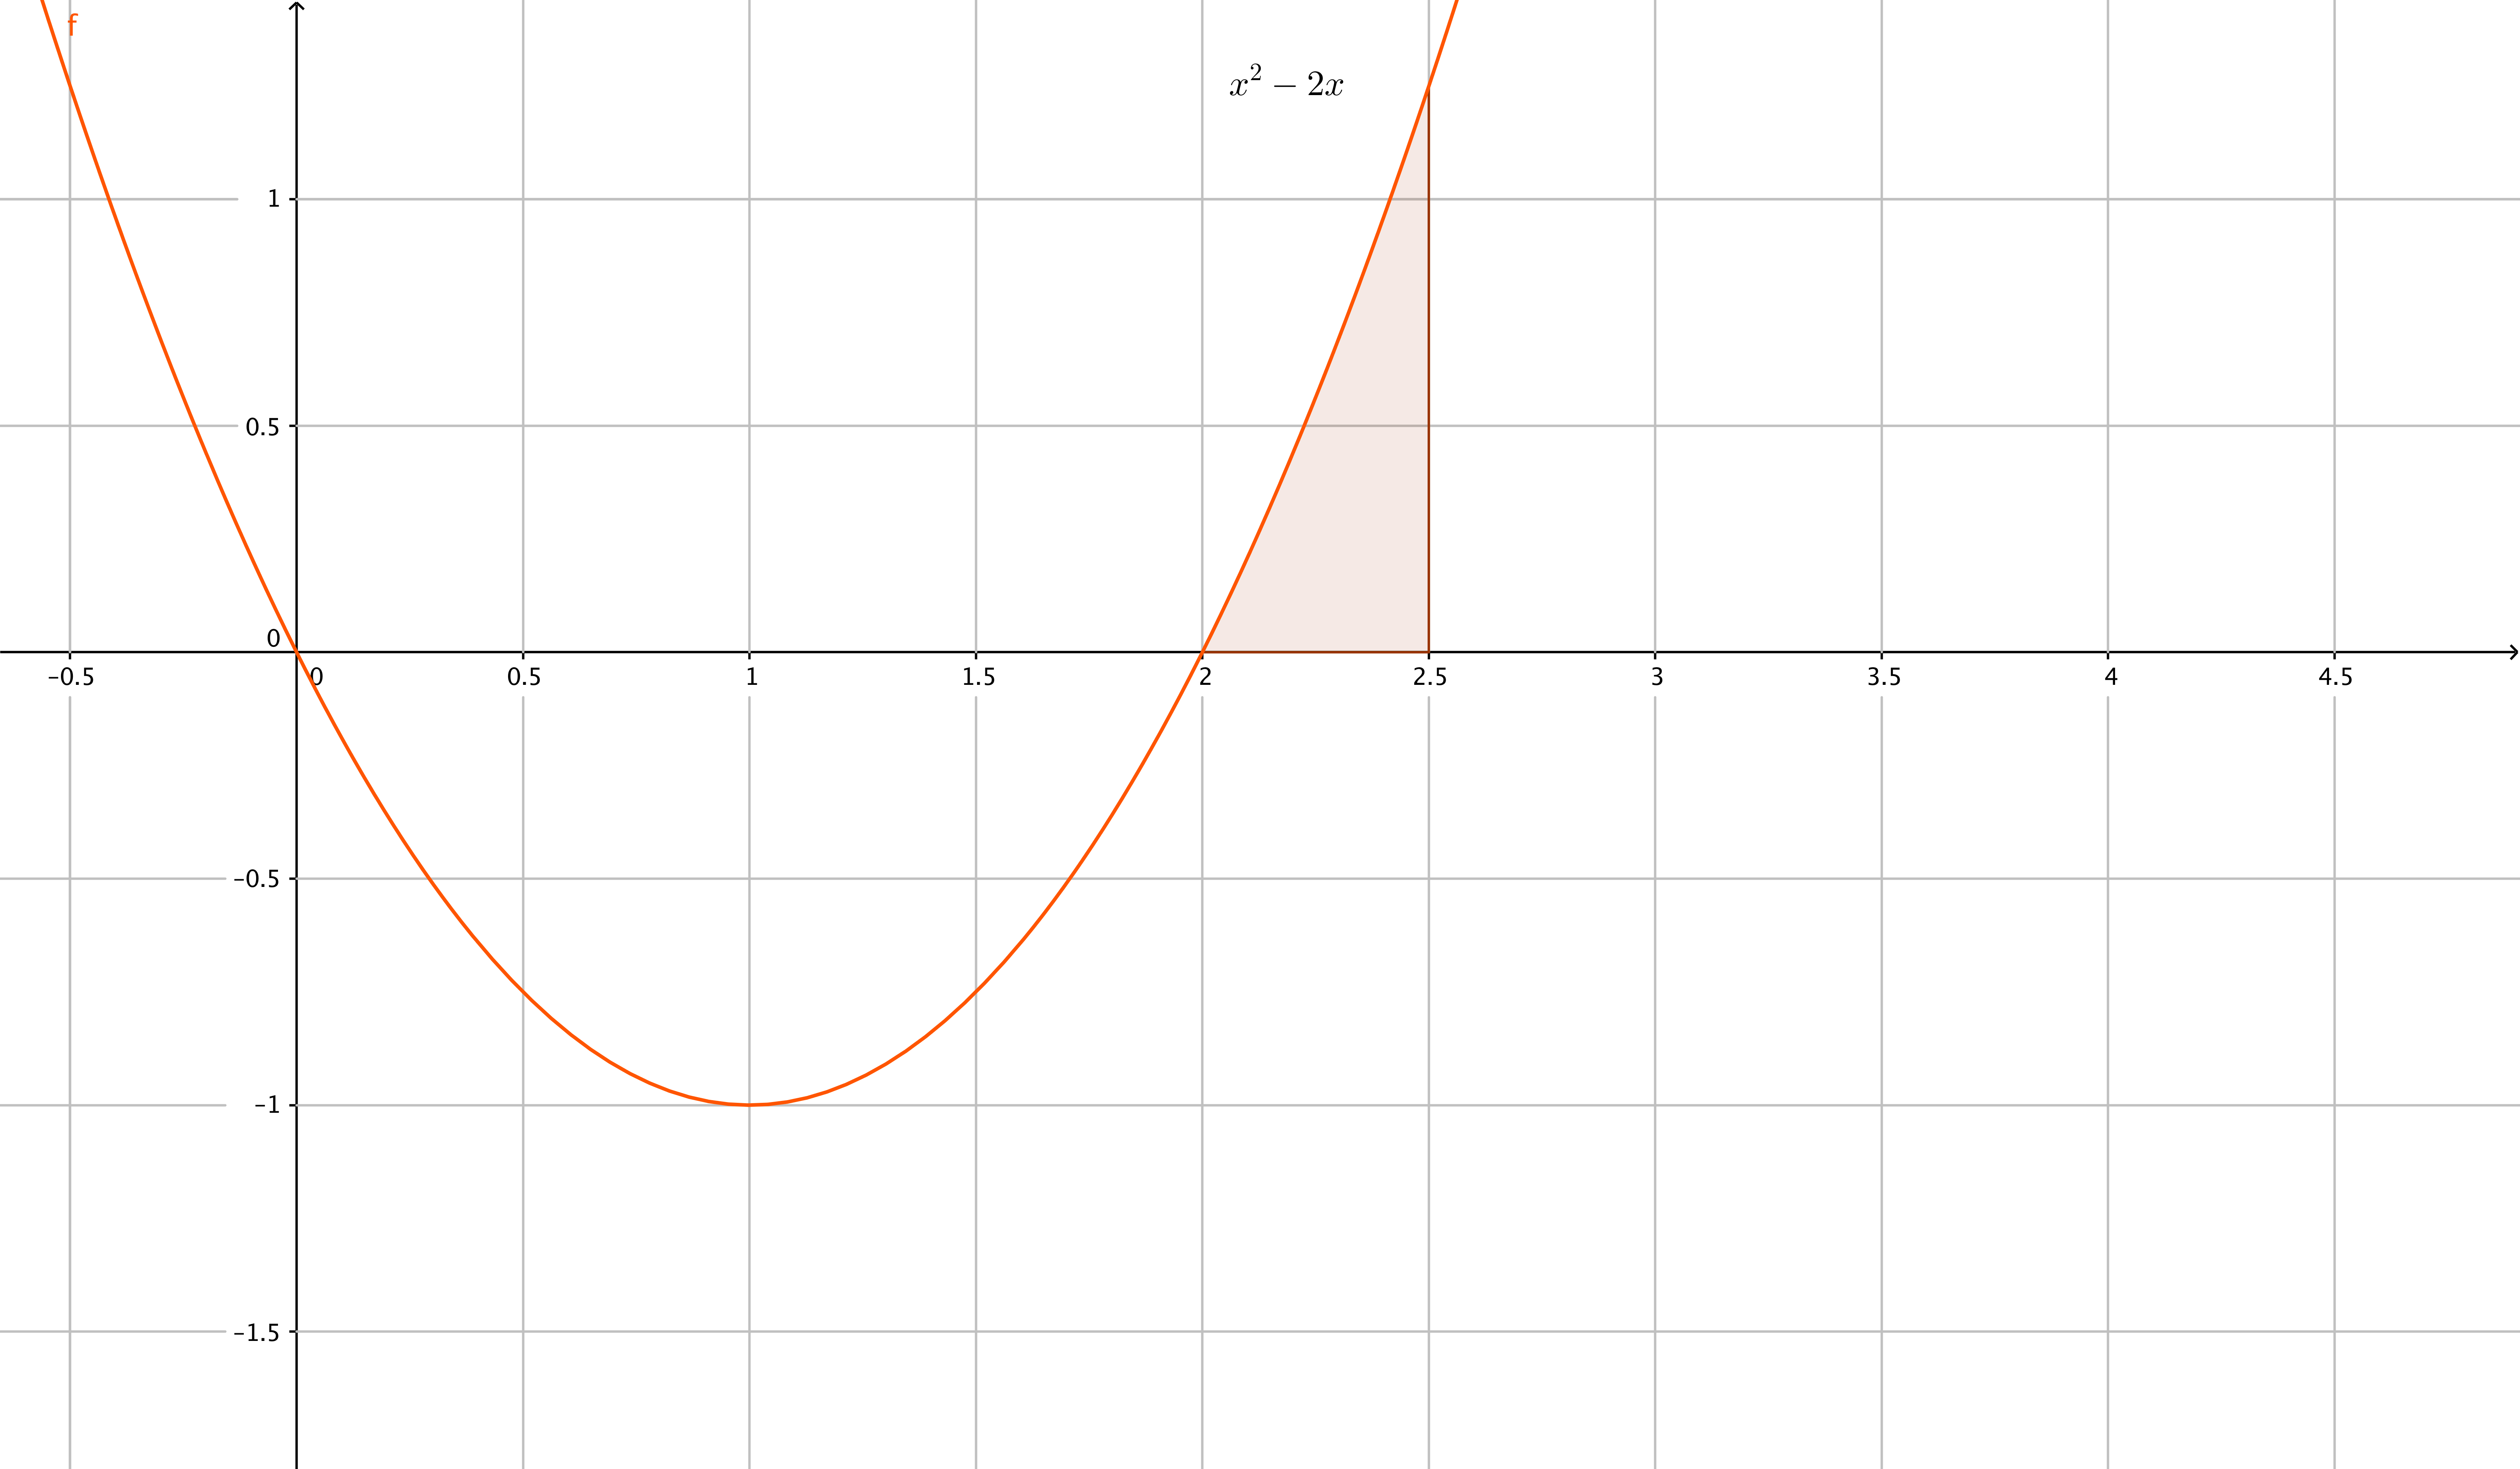
\includegraphics[width=300px, height=200px]{Integral_1.png}
	%\includegraphics[width=300px, height=200px]{Ableitung_1.png}
	\caption{}
	\end{figure}
	\end{minipage} \hfill

	\begin{minipage}{0.5\textwidth}
	Die Flaeche ueber der Abszisse und unter einer Kurve laesst sich mit Hilfe des Integrals leicht berechnen.\\
	\textbf{Beispiel}\\\\
	Um die Flaeche der Funktion $f(x)=x^2-2x$ im Intervall [2;2,5] zu berechnen muss zuert das Integral gebildet werden,
	dieses lautet $\int f(x)=F(x)=\frac{1}{3}x^3-1x^2+c$, nun setzen wir die Intervallgrenzen ein um die Flaeche zu berechnen.\\
	$F(2,5)-F(2)=\frac{1}{3}*2,5^3-1*2,5^2-\frac{1}{3}*2^3-1*2^2=0,29FE$

	\end{minipage}


	\subsubsection{Gemischte Flaechen}
	Falls die zu berechnende Flaeche sich jedoch zum Teil unter der Abszisse befindet, muss man beachte das
	man nicht ueber Abszissenschittpunkte integrieren darf d.h. befindet sich in dem zu bestimmmenden Intervall eine
	Nullstelle der Funktion muss man diese als Integrationsgrenze benutzen.\\
	\textbf{Beispiel}\\\\
	Flaeche der Funktion $f(x)=x^2-2x$ im Intervall $[0;2,5]$.\\
	Nun berechnet man die Nullstellen um herrauszufinden ob sie im Intervall liegen.\\
	\begin{align*}
	0=&x^2-2x\\
	0=&x(x-2)\\
	x_1=&0,x_2=2
	\end{align*}\\
	Da $2$ im Intervall liegt muss sie als Integrationsgrenze benutzt werden d.h. fuer die Flaeche gilt
	$A=-\int f(x)+\int f(x)=-(F(2)-F(0))+F(2,5)-F(2)=1,63FE$, da die Flaeche unter der Abszisse negativ ist muss man hier das Vorzeichen beachten.\\
	\subsubsection{Flaeche zwischen Kurven}
	Falls man die Flaeche zwischen zwei Funktionen berechnen soll, muss man falls sich Schittpunkte der Graphen im Intervall befinden
	diese als Integrationsgrenzen benutzen.\\
	\textbf{Beispiel}\\\\
	Flaeche zwischen den Funktionen $f(x)=0,25x^2$ und $g(x)=0,3x$ im Intervall $[0;1,6]$\\
	\begin{minipage}{0.3\textwidth}
	\begin{figure}[H]
	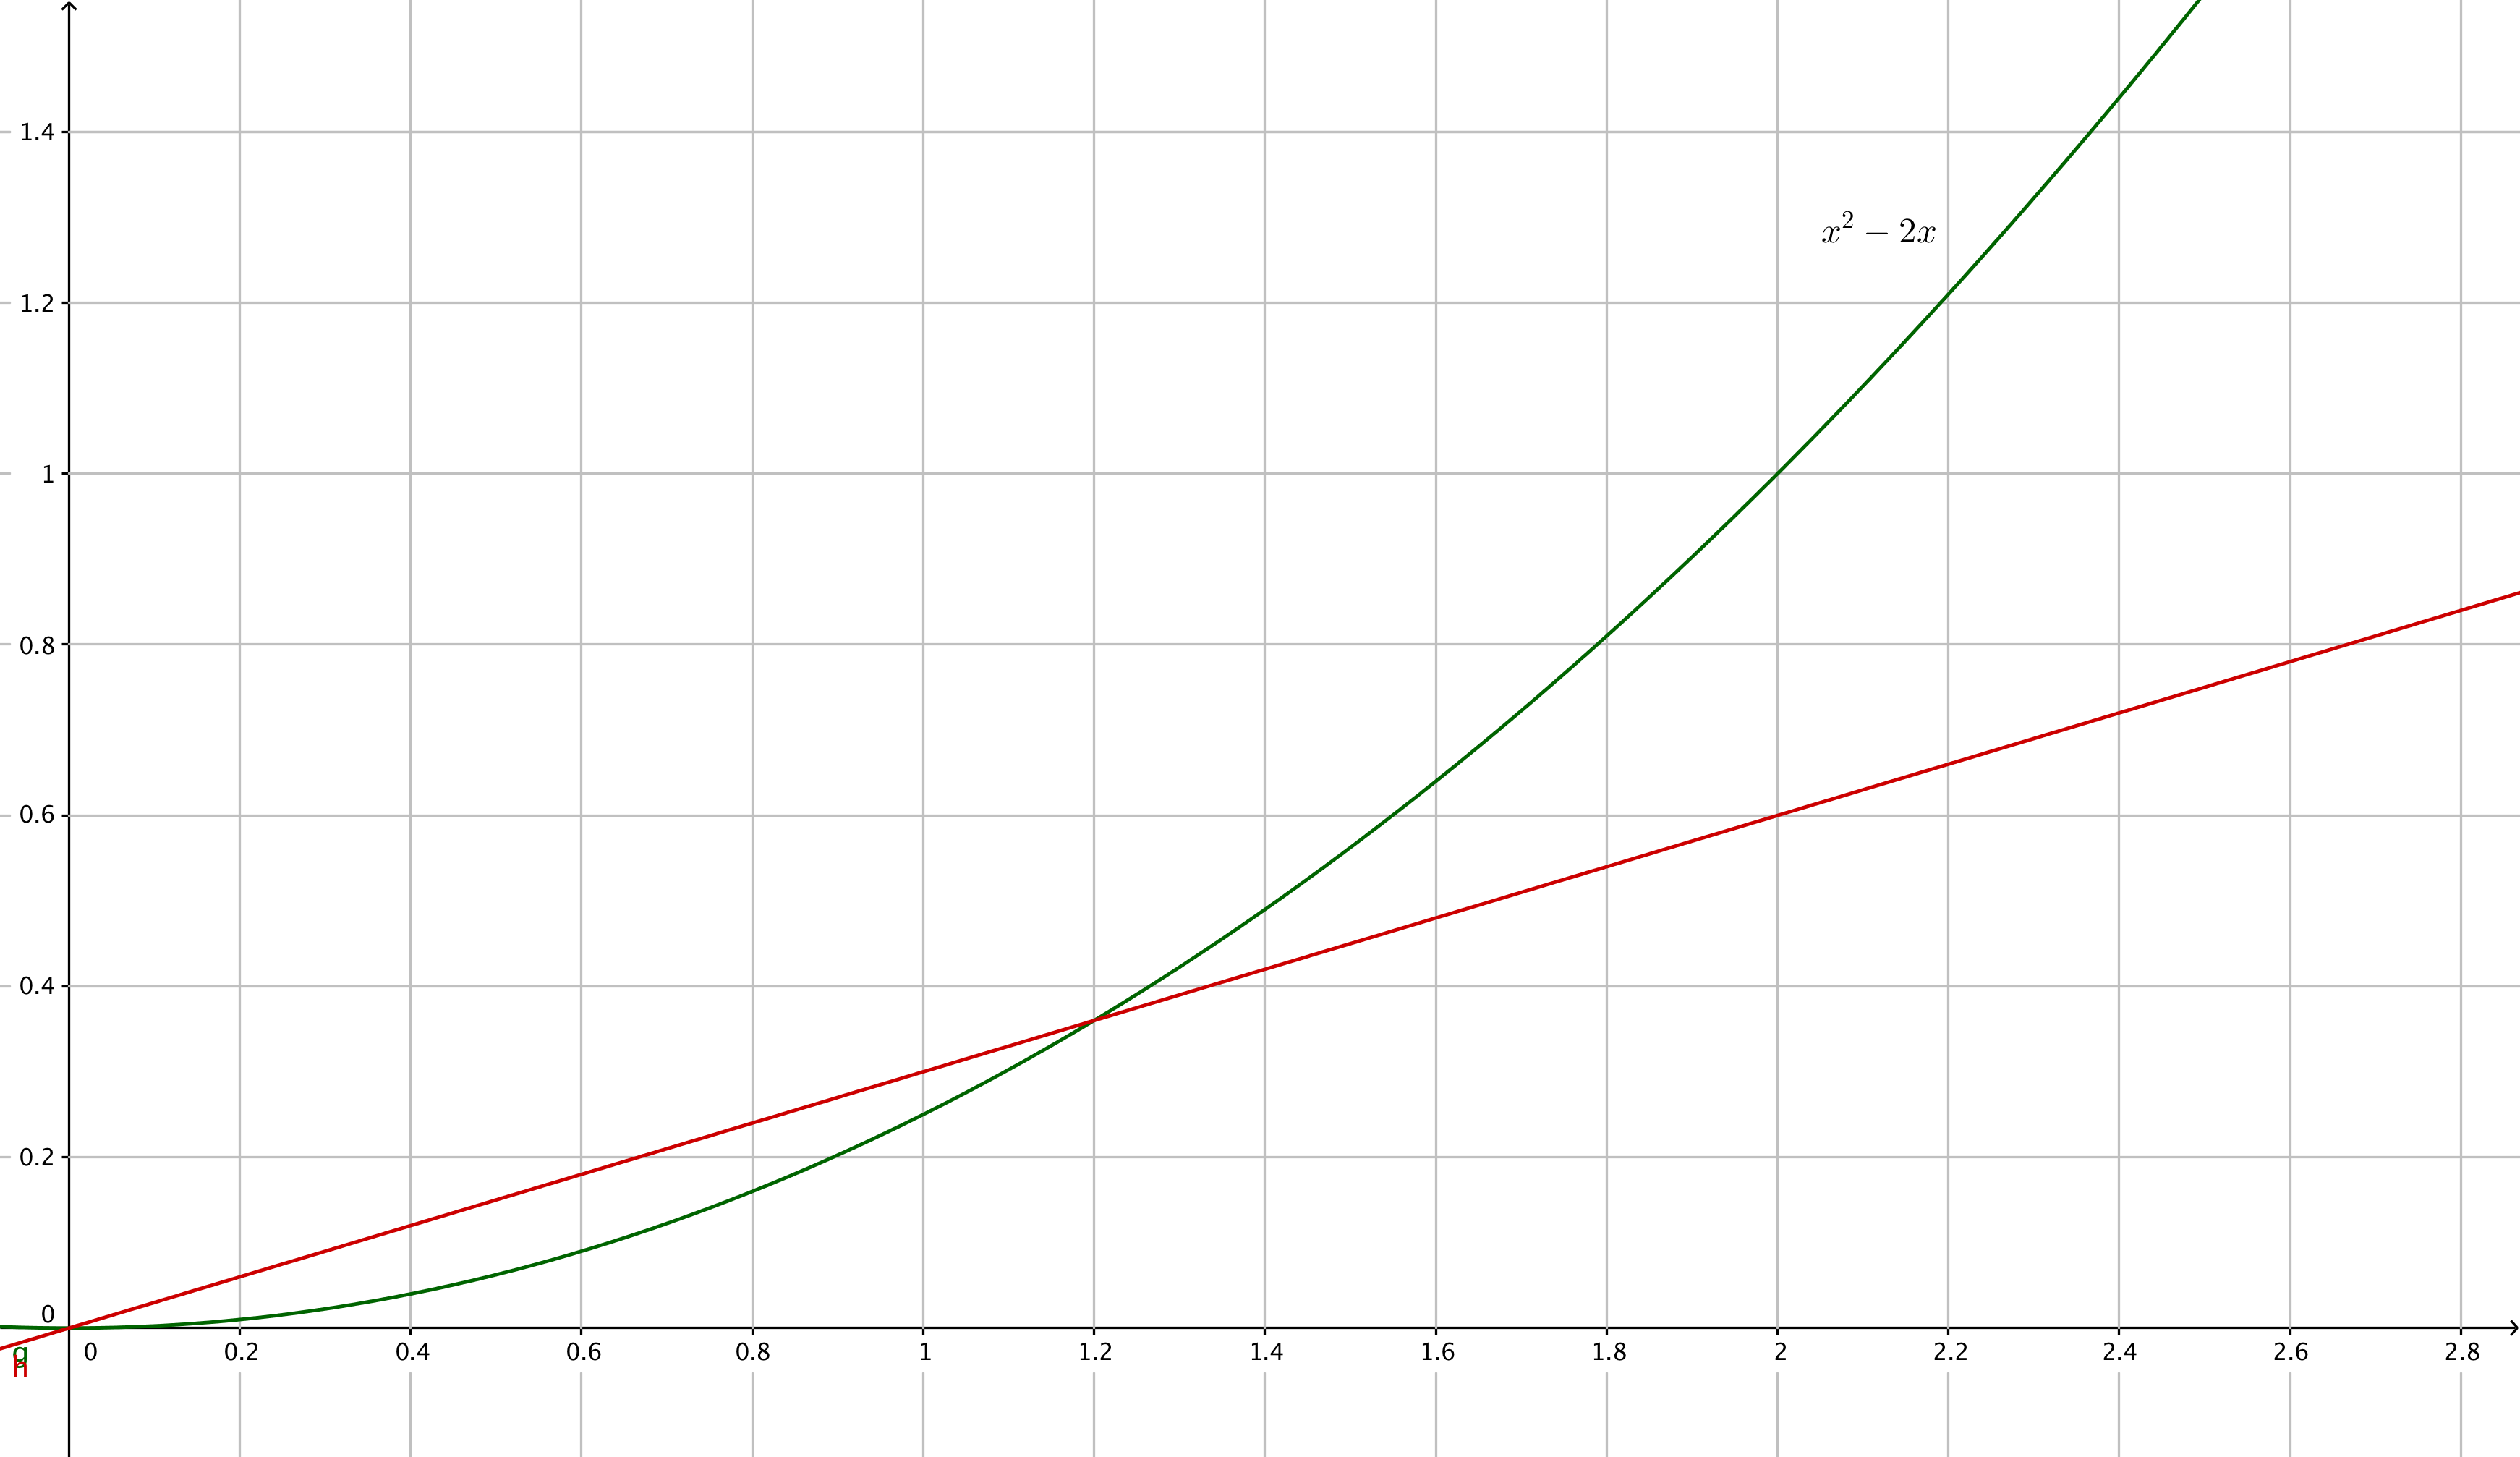
\includegraphics[width=300px, height=200px]{Integral_2.png}
	%\includegraphics[width=300px, height=200px]{Ableitung_1.png}
	\caption{}
	\end{figure}
	\end{minipage} \hfill
	\\Nun muss man herrausfinden ob sich die Graphen im Intervall schneiden.\\

	\begin{align*}
	f(x)&=g(x)\\
	0,25x^2&=0,3x|-0,3x\\
	0,25x^2-0,3x&=0|*4\\
	x^2-1,2x&=0\\
	x(x-1,2)&=0\\
	x_1&=0,x_2=1,2
	\end{align*}
	\\Da sich $1,2$ im Intervall liegt muss sie als Integrationsgrenze benutzt werden.\\
	$A=\int (g(x)-f(x))+\int (f(x)-g(x))=((G(1,2)-G(0))-(F(1,2)-F(0))+((F(1,6)-F(1,2))-(G(1,6)-G(1,2))=$\\
	Falls die Funktion zusaetzlich noch die Abszisse schneidet muss auch dieser Schnittpunkt eine Integrationsgrenze sein.
	\subsection{Mittelwert einer Funktion}
	Um den Mittelwert der Funktion f(x) im Intervall $[a;b]$ mit Hilfe des Integrals zu bestimmen, muss man die Formel
	$\frac{1}{b-a}\int\limits_{a}^{b} f(x)dx$  benutzen.
	%Sekante Integral
	\subsection{Rotationskoerper}
	Fuer das Rotationsvolumen eines Graphen um die Abszisse gilt die Formel $V = \pi*\int\limits_{a}^{b}(f(x))^2dx$\\
	\textbf{Beachte} fuer das Volumen zwischen zwei Graphen gilt \textbf{nicht} die Formel $V = \pi*\int\limits_{a}^{b}(f(x)-g(x))^2dx$
	sondern $V = \pi*\int\limits_{a}^{b}(f(x)^2-g(x)^2)dx$
	%\subsection{Herleitungen}
	%\subsubsection{Flaeche mit Hilfe des Riemann-Integrals}
	\section{Kurvendiskussion}
	\subsection{Symmetrie}
	Um herauszufinden ob eine Funktion Y-Achsensymmetrisch oder Ursprungspunktsymmetrisch ist, muss man die Exponenten einer Funktion betrachen, falls alle Exponenten einer Funktion gerade sind ist sie Achsensymmetrisch, sonst ist die Funktion Ursprungspunktsymmetrisch. Trifft keiner der beiden Bedingungen auf die Funktion zu laesst sich ihre Symmetrie nicht bestimmen.
	\begin{align*}
	& Achsensymmetrie:  & f(x)&=f(-x)\\
		& Ursprungspunktsymmetrie:  & f(x)&=-f(x)
	\end{align*}
	\subsection{Verhalten im Unendlichen}
	Das Verhalten in Unendlichen haengt vom hoechsten Exponenten und dem zugehoerigen Koeffizienten der Funktion ab, ist der Exponent gerade und der Koeffizient positiv, verlaueft die Funktion vom 2. zum 1. Quadranten, also von positiv unendlich nach positiv unendlich, ist der Koeffizient jedoch negativ, verlaueft die Funktion vom 3. zum 4. Quadranten, also von negativ unendlich nach negativ unendlich.\\
	Ist der Exponent ungerade und der Koeffizient positiv verlaueft die Funktion vom 3. zum 1. Quadranten also negativ unendlich nach positiv unendlich, ist der Koeffizient jedoch negativ verlaueft sie von 2. zum 4. Quadranten also von positiv unendlich nach negativ unendlich.\\
	Formal: \\
	Falls der hoechste Exponent ungerade und positiv ist gilt fuer $x\rightarrow\infty+ = f(x)\rightarrow\infty+$\\
	\hspace*{8.9cm} 	$x\rightarrow\infty- = f(x)\rightarrow\infty-$\\\\
	%Falls der hoechste Exponent ungerade und negativ ist gilt fuer $x\rightarrow\infty+ = f(x)\rightarrow 0$\\\\
	%\hspace*{8.9cm} 	$x\rightarrow\infty- = f(x)\rightarrow\infty-$\\
	Falls der hoechste Exponent gerade und positiv ist gilt fuer $x\rightarrow\infty+ = f(x)\rightarrow\infty+$\\
	\hspace*{8.5cm} 	$x\rightarrow\infty- = f(x)\rightarrow\infty+$\\
	\textbf{Beachte} den Koeffizienten vor dem hoechsten Exponenten!

	%\begin{align*}
	%\end{align*}

	\subsection{Schnittpunkt mit der y-Achse}
	Um den Schnittpunkt mit der Y-Achsen herauszufinden, muss man die Variable der Funktion 0 setzen.
	\subsection{Nullstellen}
	Um die Nullstellen einer Funktion zu berechnen muss man die Funktion = $0$ setzen und die dadruch enstandene Gleichung nach der Variable aufloesen.
	\subsection{Ableitungen}
	\subsection{Extrema berechnen}
	Um die Extrema einer Funktion zu erhalten muss ihre erste Ableitung $0$ gesetzt werden, nun muss man die Punkte in die 2. Ableitung
	einsetzen um herrauszufinden ob es um einen Hoch(Maximum) -oder Tiefpunkt(Minimum) handelt. Ist das Ergebnis des letzten Schrittes groesser 0
	handelt es sich um ein lokales Minimum, andernfalls handelt es sich um ein lokales Maximum. Besitzt die Funktion jedoch keine 2. Ableitung muessen die Umgebungswerte der Steigung der Punkte betrachtet werden, wechselt die Steigung von negativ zu positiv hat man ein lokales  Minimum, sonst ein lokales Maximum, um nun herrauszufinden ob ein globales Extrema vorliegt muessen alle loaklen Extrema verglichen werden.\\\\
	\begin{align*}
		&Notwendige\enspace Bedingung\enspace &f'(x_0)&=0\\
		&Hinreichende\enspace Bedingung\enspace Hochpunkt\enspace &f''(x_0)&<0\enspace \lor \enspace f'(x_0)+\rightarrow f'(x_0)- \\
		&Hinreichende\enspace Bedingung\enspace Tiefpunkt\enspace &f''(x_0&>0\enspace \lor \enspace f'(x_0)+\rightarrow f'(x_0)-
	\end{align*}
	\subsection{Wendepunkte berechnen}
	Um die Wendepunkte einer Funktion zu berechen muss die 2. Ableitung 0 gesetzt werden, um nun zu ueberpruefen ob der Punkt ein Sattelpunkt ist muss falls die Funktion eine 3. Ableitung besitzt diese an dem vorher berechneten Punkt $\neq 0$ sein, ist die 3. Ableitung nicht vorhanden muss an diesem Punkt ein Vorzeichenwechsel stattfinden.
	\begin{align*}
		&Notwendige\enspace Bedingung\enspace &f''(x_0)&=0\\
		&Hinreichende\enspace Bedingung\enspace Wendepunkt\enspace &f'''(x_0)& \neq 0\enspace \lor \enspace f''(x_0)\pm\rightarrow f''(x_0)\mp \\
	\end{align*}
	\pagebreak
	\section{Analytische Geometrie}
	\subsection{Was ist ein Vektor}
	Ein Vektor ist eine Menge von Pfeilen der Form $\vec{a} = \begin{pmatrix} a_1 \\ \vdots \\ a_n \end{pmatrix} $, die parallel untereinander verschoben sind.
	Eine anderen Notation fuer diesen Vektor waere $\vec{a} = \begin{pmatrix} a_1  \hdots  a_n \end{pmatrix}^T $
	\subsection{Koordinatensystem}
	\begin{minipage}{0.5\textwidth}
			\begin{figure}[H]
				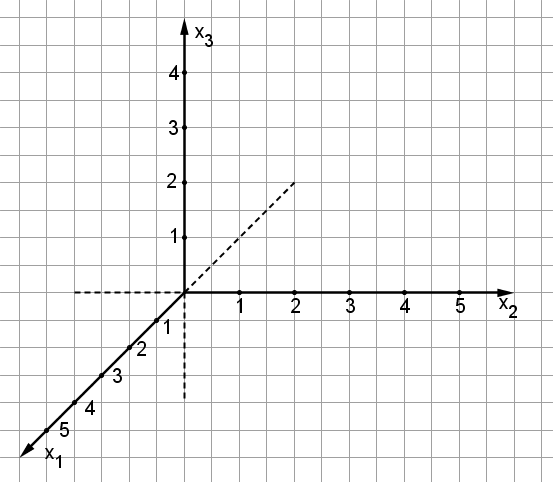
\includegraphics[width=200px, height=200px]{koordinatensystem.png}
					\captionsetup{labelformat=empty}
				\caption{3D Koordinatensystem}
			\end{figure}
		\end{minipage}
	\subsection{Besondere Vektoren}
	\subsubsection{Nullvektor}
	Der Nullvektor ist ein Vektor der Form $\vec{v} = \begin{pmatrix} 0 \\ \vdots \\ 0 \end{pmatrix}$,
	 zudem ist er das neutrale Element der Vektoraddition d.h. $ \vec{a} + \begin{pmatrix} 0 \\ \vdots \\ 0 \end{pmatrix} = \vec{a}$.
	\subsubsection{Gegenvektor}
	Der Gegenvektor ist das inverse Element der Vektoraddtion d.h $ \vec{a}+ -\vec{a}=\vec{0}$, wobei $\vec{0}$ den Nullvektor bezeichnet.
	\subsubsection{Ortsvektor}
	Ein Ortsvektor bezeichnet einen Vektor der vom Koordinatenursprung aus geht d.h. er hat die Form $\vec{OP}$, wobei $P$ ein beliebiger Punkt im Raum ist.
	\subsubsection{Normalenvektor}
	Ein Normalenvektor ist ein Vektor der orthogonal zu seinem Bezugsobjekt z.B. einer Gerade ist.
	\subsubsection{Einheitsvektor}
	Ein Einheitsvektor ist ein Vektor der Laenge 1, d.h. dass sein Betrag = 1 ist($|\vec{a}|=1$).
	\\\\\textbf{Beispiel}\\
	Der Einheitsvektor $\vec{e_a}$ des Vektors $\vec{a}$ wird berechnet indem man $\frac{\vec{a}}{|a|}$ rechnet.
	\subsection{Rechnen mit Vektoren}
	\subsubsection{Addition}
	Zwei Vekotren in $\mathbb{R}^3$ $\vec{a}, \vec{b}$ werden addiert, idem man ihre Komponenten addiert.
	\\Beipsiel\\
	\begin{align*} \vec{a}+\vec{b}=\begin{pmatrix}a_1\\a_2\\a_3\end{pmatrix}+\begin{pmatrix}b_1\\b_2\\b_3\end{pmatrix}=\begin{pmatrix}a_1+b_1\\a_2+b_2\\a_3+b_3\end{pmatrix} \end{align*}
	\subsubsection{s-Multilipkation}
	Ein Vektor $\vec{a}$ aus $\mathbb{R}^3$  wird mit einer Zahl $s$ aus $\mathbb{R}$ multipliziert, in dem seine Komponenten mit $s$ multipliziert werden.\\Beispiel
	\begin{align*}  s*\vec{a}=s*\begin{pmatrix}a_1\\a_2\\a_3\end{pmatrix}=\begin{pmatrix}s*a_1\\s*a_2\\s*a_3\end{pmatrix} \end{align*}
	\subsubsection{Linearkombination}
	Einen Ausdruck der Form $r_1*\vec{a}_1 + r_2*\vec{a}_2 + \hdots + r_n*\vec{a}_n $ nennt man Linearekombination der Vektoren $a_1$ bis $a_n$.
	Beachte das $a_1$ bis $a_n$ keine Vektorkomponenten sondern Vektoren sind.
	\subsubsection{Laenge eines Vektors}
	Der Betrag eines Vektors $\vec{a}$ stellt seine Laege da, d.h. $|a|=\sqrt{a_1^2+a_2^2+a_3^2}$ ist die Laenge eines Vektors.
	\subsubsection{Lineare Abhaengigkeit}
	Die Lineare Anhaenigkeit beschreibt die Eigenschaft eines Vektors $\vec{v}$ sich mit Hilfe der s-Multiplikation und eines beliebigen Vektors $\vec{b}$ herstellen zu lassen.
	\\\\Beispiel:
	\begin{align*} \vec{v}=s*\vec{b} \end{align*}
	Falls es ein $s$ in $\mathbb{R}$ gibt das die Gleichung erfuellt ist $\vec{v}$ linear Abhaengig von $\vec{b}$.
	\subsubsection{Skalarprodukt}
	Das Sklalarprodukt ordnet je zwei Vektoren $\vec{a},\vec{b}$ ein Sklalar zu, ist dieses Skalar $0$ sind die Vektoren orthogonal zueinander.\\\\Beispiel  \begin{align*} \vec{a} \circ \vec{b}=a_1*b_1+a_2*b_2+a_3*b_3. \end{align*}
	\subsubsection{Kreuzprodukt}
	\paragraph{Berechnung mithilfe der Determinante}
	\hspace{0 cm} \\ \noindent \\
	Das Kreuzprodukt leasst sich auch mithilfe der Determinante berechnen indem man, eine quadr. Matrix mit der Standardbasis und zwei sich schneidende Vektoren
	bildet.\\\\
	$\begin{array}{cc}
	\vec{a} x \vec{b}=det\begin{pmatrix} e_1 & a_1 & b_1 \\ e_2 & a_2 & b_2  \\ e_3 & a_3 & b_3  \end{pmatrix}
	&= e_1\left|\begin{array}{cc} a_2 & b_2 \\ a_3 & b_3\end{array} \right|-e_2\left|\begin{array}{cc} a_1 & b_1 \\ a_3 & b_3\end{array} \right|+e_3\left|\begin{array}{cc} a_1 & b_1 \\ a_2 & b_2\end{array} \right|\\
	&= e_1\left|\begin{array}{cc} a_2 & b_2 \\ a_3 & b_3\end{array} \right|+e_2\left|\begin{array}{cc} a_3 & b_3 \\ a_1 & b_1\end{array} \right|+e_3\left|\begin{array}{cc} a_1 & b_1 \\ a_2 & b_2\end{array} \right|\\
	&= e_1(a_2*b_3-a_3*b_2)+e_2(a_3*b_1-a_1*b_3)+e_3(a_1*b_2-a_2*b_1)\\
	&=\begin{pmatrix} e_1 \\ e_2 \\ e_3 \end{pmatrix} \circ \begin{pmatrix} a_2*b_3-a_3*b_2 \\ a_3*b_1-a_1*b_3 \\ a_1*b_2-a_2*b_1 \end{pmatrix}
	\end{array}$
	\\Der hintere Teil entspricht nun dem Kreutzprodukt.
	%Be\subsubsection{Spatprodukt}
	\subsection{Geraden}
	\subsubsection{Was sind Geraden}
	Eine Gerade im 3-Dimensionalen Raum ist eine unendliche Ausdehnung in eine Koordinatenrichtungen.
	\subsubsection{Lage von zwei Geraden im Raum}
	Um die Lage zweier Gerade zueiander zu bestimmen muss zuert auf lineare Anhaengigkeit geprueft werden.
	Sind die Richtungsvektoren linear Abhaengig, sind die Gerade etweder Parallel oder Identisch, sind sie jedoch linear Unabhaengig
	muss geprueft werden ob sie einen Schnittpunkt besitzen oder windschief sind.
	\\\\Beispiel \textbf{Parallel}
	\\Fall wir herrausgefunden haben dass die Richtungsvektoren lineare Abhaengig sind, muessen wir als naechstes schauen ob der Ortsvektor einer beteiligten Gerade auf der anderen Gerade liegt um zu pruefen ob die Gerade Identisch sind.
	\\\\Beispiel \textbf{Windschief}
	\\Hat sich jedoch ergeben dass die Richtungsvektoren linear  Unabhaengig sind, muess wird als naechstes schauen die Geraden einen Schnittpunkt besitzen um zu pruefen ob sie windschief sind.
	\paragraph{Abstand Punkt Gerade}
	\hspace{0 cm} \\ \noindent \\
	Um den Abstand von einem Punkt($\vec{p}$) zu einer Geraden($g: \vec{x}=\vec{o}+r*\vec{s}$) berechnen, bilden wir einen Vektor von einem beliebingen Punkt auf der Gerade zu dem Punkt zu dem wir den Abstand berechnen wollen. Nun berechnen wir den Betrag von Kreuzprodukt dieses Vektors und dem Richtungsvektor von $g$, dies stell die Flaeche des Parallelogramms dar das sie aufspannen,
	da die Flaecheformdel des Parallelogramms $A=g*h$ ist berechnen wir nun den Betrag des Richtungsvektors von $g$ und stellen die Flaechenformel nach $h$ um, dann setzen wir die Werte ein die wir eben berechnet haben ein.
	%\\\textbf{Abstand mit Hilfe der 2D-HNF}
	\paragraph{Abstand Gerade Gerade}
	\hspace{0 cm} \\ \noindent \\
	\textbf{Windschief\\}
	Der Abstand von zwei windschiefen Geraden laesst sich mit Hilfe einer Hilfsebene berechnen, indem man zuerst den Normaleneinheitsvektor der beiden Richtungsvektoren berechnet, nun kann man die Hessesche Normalenform verwenden um den Abstand zu berechnen.\\\\
	Beispiel\\
	\textbf{Parallel\\}
	Siehe Abstand Gerade Punkt, wobei der Punkt ein beliebiger Punkt der 2. Gerade ist.
	\paragraph{Winkel zwischen Geraden}
	\hspace{0 cm} \\ \noindent \\
	Seien die Gerade $g_1: \vec{x}= \vec{o_1}+r*\vec{a}$ und $ g_2: \vec{x}=\vec{o_2}+s*\vec{b} $  geschnitten, dann berechnet sich der Winkel zwischen ihnen folgendermassen:
	\begin{align*}
		cos(\phi)= \frac{\vec{a} \circ \vec{b}}{|\vec{a}|*|\vec{b}|}
	\end{align*}
	\subsection{Ebenen}
	Eine Ebene im 3-Dimensionalen Raum ist eine unendliche Ausdehnung in zwei Vektorrichtungen.
	\begin{figure}[H]
				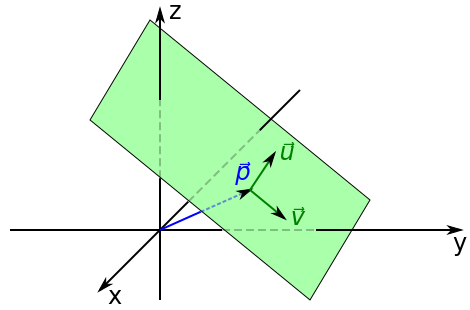
\includegraphics[width=150px, height=150px]{Ebene.png}$^{[5]}$
					\captionsetup{labelformat=empty}
				\caption{Ebene im 3-Dimensionalen Raum}
	\end{figure}
	\subsubsection{Ebenenformen}
	\paragraph{Parameterform}
		\hspace{0 cm} \\ \noindent \\
	Paramterform einer Ebene: $E : \vec{x} = \vec{p}+ r*\vec{u}+s*\vec{v}$\\
	In der Paramterform wird eine Ebene mithilfe eines Stuetzvektors(Ortsvektors) und zwei Richtungsvektoren beschrieben.
	Es gibt zwei Moeglichkeiten wie diese Richtungsvektoren zueiander liegen duerfen um eine Ebene zu beschreiben,echt parallel und geschnitten. Falls sich die gegebenen Richtugnsvektoren schneiden, kann die Ebene direkt zwischen ihnen aufgespannt werden.
	Falls die gegeben Richtungsvektoren jedoch echt parallel sind, muss ein Verbindungsvektor zwischen ihen hergestellt werden, wobei einer der beiden echt parallelen Richtungsvektoren ausgetauscht werden muss.
	\\\\\textbf{Beispiel}\\
	Fuer die Pruefung ob die Gerade Parallel sind siehe Lage Gerade Gerade.\\
	Seien die Gerade $g_1: \vec{x}= \vec{o_1}+r*\vec{a}$ und $ g_2: \vec{x}=\vec{o_2}+s*\vec{b} $ echt parallel,
	dann kann die Ebene mit Hilfe des Richtungsvektors von einer der Geraden und eines beliebigen Verbindungsvektors der zwei Geraden gebildet werden.
	\paragraph{Normalenform}
		\hspace{0 cm} \\ \noindent \\
		Normalenform einer Ebene $E : 0 = \vec{n}\circ\left[\left(\vec{x}-\vec{p}\right)   \right]$\\
		In der Normalenform wird eine Ebene mit Hilfe ihrer Normale($\vec{n}$) und der Differenz eines Punktes aus der Ebene mit einem beliebigen anderen Punkt beschrieben($\vec{x}-\vec{p}$) wobei $\vec{p}$ einen beliebigen Punkt in der Ebene, und $\vec{x}$ einen beliebigen anderen Punkt darstellt. Alle Differenzen die orthogonal zum Normalenvektor der Ebene liegen beschreiben daher Vektoren die in der Ebene liegen.

	\paragraph{Koordinatenform}
		\hspace{0 cm} \\ \noindent \\
		Koordinatenform der Ebene: $E: n_1*x_1+n_2*x_2+n_3*x_3=c$\\
		Die Koordinatenform der Ebene ist die ausmultiplizierte Normalenform einer Ebene.
		\\\\Beispiel
	\paragraph{Hessesche Normalenform(HNF)}
	\hspace{0 cm} \\ \noindent \\
	HNF einer Ebene $E : d = \vec{n_0}\circ\left[\left(\vec{x}-\vec{p}\right)   \right]$\\
	Die HNF ist eine abgewandelte Form der Normalenform, sie unterscheidet sich dadurch das ihr Normalenvektor($\vec{n_0}$)
	normiert ist, d.h er hat die Laenge 1, dadurch kann der Abstand von einer mit ihr beschrieben Ebene zu einem anderen Objekt sehr einfach durch das einsetzen dieses Objekts berechnet werden(Vektorprojektion).
	\subsubsection{Lage Ebene Gerade}
	Um die Lage einer Gerade zu Ebene zu bestimment, muss man zuert ueberpruefen ob die Gerade echt parallel ist, dies kann man mit Hilfe der Normale der Ebene und des Richtungsvektors der Gerade ueberpruefen indem man ueberprueft ob die Normale orthogonal zum Richtungsvektor der Gerade liegt.
	Fall die Gerade parallel zur Ebene liegt, kann man nun den Ortsvektor der Gerade in die Ebene einsetzen um zu ueberpruefen ob sie identisch sind.
	Falls die Gerade sich jedoch nicht parallel zur Ebene verhaelt hat sie garantiert einen Schnittpunkt mit der Ebene.
	\paragraph{Schnittpunkt}
		\hspace{0 cm} \\ \noindent \\
		Um den Schnittpunkt einer Gerade mit einer Ebene zu berechnen, bringt man die Ebene in Koordinatenform und setzt die Gerade dann in diese ein.
		\\\\Beispiel
	\paragraph{Abstand Gerade Ebene}
	\hspace{0 cm} \\ \noindent \\
	Damit eine Gerade und eine Ebene ueberhaupt einen Abstand haben, muessen sie selbstverstaendlich echt parallel sein,
	um dies festzustellen ueberprueft man den Normalenvektor der Ebene und den Richtungsvektor der Gerdade auf orthogonalitaet.
	Falls die Orthogonalitaetsbedingung erfuellt ist, waehlt man nun ein beliebigen Punkt auf der Ebene und bildet mit der Hilfe von
	diesem Punkt und der Normale der Ebene eine Gerade, nun berechnet man den Schnittpunkt von dieser Gerade mit der Ebene.
	Nun bildet man den Vektor zwischen dem Ortsvektor der neuen Gerade und de Schittpunkt der Ebene, der Betrag dieses Vektors
	ist dann der Abstand von der Gerade zur Ebene.\\\\
	\textbf{Abstand ohne die HNF}\\
	\textbf{Abstand mit Hilfe der HNF}\\
	Siehe Abstand Ebene Ebene, wobei der Punkt ein beliebiger der Geraden sein kann.

	\paragraph{Winkel zwischen Gerade und Ebene}
	\hspace{0 cm} \\ \noindent \\
	Sei die Gerade $g_1: \vec{x}= \vec{o_1}+r*\vec{a}$ nicht parallel zu $E : \vec{x} = \vec{p}+ r*\vec{u}+s*\vec{v}$, dann existiert ein Winklel($\phi$) zwischen ihnen, der sich mit Hilfe der Normalenvektors der Ebene($\vec{n}$) folgendermassen berechnen laesst:
	\begin{align*}
		sin(\phi)= \frac{|\vec{a} \circ \vec{n}|}{|\vec{a}|*|\vec{n}|}
	\end{align*}
	\textbf{Bermerkung:}
	Ergibt sich $sin(\phi)=0$, ist die Gerade parallel oder identisch zu der Ebene.
	\subsubsection{Lage Ebene Ebene}
	Um die Lage einer Ebene zu einer anderen Ebene stellt man zuerst fest ob sie parallel zueiander liegen, dies kann man ueberprufen indem man die beiden Normalen der Ebene auf lineare Abhaengigkeit ueberprueft.
	\paragraph{Identisch}
		\hspace{0 cm} \\ \noindent \\
	Um nun zu ueberpruefen ob die Ebenen identisch sind, setzt einen belibigen Punkt der einen Ebene in die andere Ebene ein.
	(Koennte Schnittgerade sein, Loesung 3 Punkte einsetzen die zusammen keine Gerade bilden koennen)
	\paragraph{Schnittgerade}
	Um die Schnittgerade zweier Ebenen zu berechen, bietet es sich an eine der Ebene in die Kooridantenform umzuwandeln,
	nun kann man einfach $x1$ bis $x3$ in die Koordinatenform einsetzen und solange umstellen bis sich eien Variable durch die anderen ersetzen laesst, nun setzt man die berechnete Gleichung in die Ebene in Parameterform ein und erhaelt so eine Schnittgerade.
	\paragraph{Abstand Ebene Ebene}
		\hspace{0 cm} \\ \noindent \\
	\textbf{Abstand ohne die HNF}\\
	Um den Abstand zweier Ebenen zu berechnen muessen diese selbstverstaendlich parallel zueiandern liegen, nun berechnet man von einer der Ebenen die Normale und stellt mit ihrer Hilfe eine Gerade auf, dann berechnet man den Schnittpunkt dieser Gerade mit der anderen Ebene.\\
	Nun berechnet man den Vektor zwischen dem Ortsvektor der Normale und dem Schnittpunkt, der Betrag dieses Vektors ist der Abstand zwischen den beiden Ebenen.\\\\
	\textbf{Abstand mit Hilfe der HNF}\\
	Da zwei Ebene parallel zueiander liegen muessen um einen Abstand zu haben, kann man um den Abstand von zwei Ebenen einfach berechnen indem man einen belibiegen Punkt der einen Ebene in die HNF der anderen einsetzt.
	\paragraph{Winkel zwischen Ebenen}
	\hspace{0 cm} \\ \noindent \\
	Seien $E_1$ und $E_2$ zwei Ebenen, dann gilt fuer ihren Schnittwinkel:
	\begin{align*}
		cos(\phi)= \frac{|\vec{n_1} \circ \vec{n_2}|}{|\vec{n_1}|*|\vec{n_2}|}
	\end{align*}\\\\
	\textbf{Bermerkung:}
	Ergibt sich $cos(\phi)=1$, sind die Ebenen parallel oder identisch.

	\subsection{Kugeln}
	\subsubsection{Was ist eine Kugel}
	Eine Kugel ist eine Menge von Punkten im 3-Dimensionalen Raum, die von einem festen Punkt $M$ den gleichen Abstand $r$ haben,
	der Punkt $M$ wird dabei als Mittelpunkt und der Abstand $r$ als Radius bezeichnet.
	\subsubsection{Kugelgleichung}
	Eine Kugel in der Analytischen Geometrie wird mit der Gleichung\\ $|\vec{p}-\vec{M}|^2=r^2$ oder
	$(p_1-M_1)^2+(p_2-M_2)^2+(p_3-M_3)^2=r^2$ beschrieben, wo $M$ den Mittelpunkt als Vektor, $p$ einen beliebigen Punkt als Vektor, und $r$ den Radius als reele Zahl darstellt.
	\subsubsection{Lage Kugel Gerade}
	Im $\mathbb{R}^3$ gibt es zwei Moeglichkeiten wie eine Gerade zu einer Kugel liegen kann, ersten wenn ie Kugel von der Geradeb geschnitten wird und zweitens wenn ebendies nicht zutrifft. Dies kann man feststellen indem man den Abstand der Gerade zum Kugelmittelpunkt berechnet, ist dieser Abstand groesser als der Kugelradius haben die Gerade und die Kugel keine gemeinsamen Punkte, ist er jedoch kleiner enstehen zwei Schnittpunkte.
	\paragraph{Abstand}
	\hspace{0 cm} \\ \noindent \\
	Siehe Abstand Punkt Gerade, wobei der Punkt den Kugelmittelpunkt darstellt.
	%\paragraph{Schnittpunkte}
	\subsubsection{Lage Kugel Ebene}
	Im $\mathbb{R}^3$ gibt es zwei Moeglichkeiten wie eine Ebene zu einer Kugel liegen kann, erstens wenn die Kugel von der Ebene geschnitten wird und zweitens wenn ebendies nicht zutrifft. Dies kann man festellen indem man den Abstand der Ebene zum Kugelmittelpunkt berechnet, ist dieser Abstand groesser als der Kugelradius haben die Ebene und die Kugel keine gemeinsamen Punkte, ist er jedoch kleiner ensteht eine Schnittkreis.
	\paragraph{Abstand}
	\hspace{0 cm} \\ \noindent \\
	Siehe Abstand Punkt Ebene, wobei die Normale den Richtungsvektor und der Kugelmittelpunkt den Ortsvektor der Gerade darstellt.
	\\\\\textbf{Beispiel}
	\paragraph{Flaeche der Schnittkreis}
	\hspace{0 cm} \\ \noindent \\
	Um die Flaeche des Schnittkreises zu berechnen muss zunaechste der Radius des Kreises berechnet werden,
	diesen kann man mit Hilfe der Entfernung der Ebene zum Mittelpunkt und des Kugelradius berechen.
	Es gilt:
	\begin{align*}
	r_{Kreis}^2 &=r_{Kugel}^2-(Abstand Kugelmittelpunkt Ebene)^2\\
	A_{Kreis} &= \pi*r_{Kreis}^2
	\end{align*}
	%\subsubsection{Tangentialebene}
	\subsubsection{Lage Kugel Kugel}
	Im $\mathbb{R}^3$ gibt zwei Moeglichkeiten wie eine Kugel zu einer anderen Kugel liegen kann, ersten wenn die eine Kugel die anderen schneidet und zweitens wenn ebendies nicht zutrifft. Dies kann man festellen indem man der Abstand der beiden Mittelpunkte berechnet, ist dieser groesser als die Summe der beiden Kugelradien haben die Kugeln keine gemeinsamen Punkte, ist er jedoch kleiner entsteht ein Schnittkoeper.
	\paragraph{Abstand}
	\hspace{0 cm} \\ \noindent \\
	Trivial(Abstand Punkt Punkt).
	\subsection{Herleitungen}
	\subsubsection{Satz des Pythagoras}
	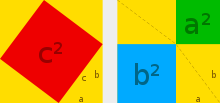
\includegraphics[width=220 px, height=103 px]{pytha.png}\\
	Links = $c^2+ 4*(\frac{1}{2}a*b)$\\
	Rechts = $a^2+b^2+4*(\frac{1}{2}a*b)$

	\begin{align*}
	c^2+ 4*(\frac{1}{2}a*b) &= a^2+b^2+4*(\frac{1}{2}a*b)  \hspace{0.5 cm} |-4*(\frac{1}{2}a*b)\\
	c^2 &= a^2+b^2
	\end{align*}




	%\subsubsection{Pythagoras im Raum}
	%\subsubsection{Kosinussatz}
	%\subsubsection{Skalarprodukt}
	%\subsubsection{Kreuzprodukt}
	%\subsubsection{Spatprodukt}
	%\subsubsection{Hessesche Normalform}
	%\subsubsection{2D-Hesse'sche Normalform}
	\section{Lineare Algebra}
	\subsection{Loesungsverfahren fuer LGS}
	\subsubsection{Treppenstuffen Verfahren}
	\subsubsection{Koeffizienten Matrix}
	\pagebreak

	\subsubsection{Determinante}
	Die Determinante einer Matrix laesst sich mit Hilfe des Laplacescher Entwicklungssatz in zwei ...Richtungs" entwickeln.\\
	$det A = \sum\limits_{i=1}^{n}(-1)^{j+i}*a_{ij}*detA_{ij} $ (Entwicklung nach der $j$-ten Spalte)\\
	$det A = \sum\limits_{j=1}^{n}(-1)^{j+i}*a_{ij}*detA_{ij} $ (Entwicklung nach der $i$-ten Zeile)\\\\
	wobei $A_{ij}$ die ${(n-1)} \times {(n-1)}$-Untermatrix von $A$ ist, um diese zu Erhalten muss jeweil die $i-te$ Zeile und die $j-te$ Spalten gestrichen werden.
	\\\\Beispiel
	\subsection{Matrizen}
	 \hspace{0 cm}
	Eine Matrix vom Typ $M_{m,n}$ ist eine Zusammenfassung von Werten der Form $M =$
	$
	\begin{pmatrix}
		a_{11} & a_{12} & ... 	& a_{1n}\\
		a_{21} & a_{22} & ...		 & a_{2n}\\
	      \vdots    	&      &	    \\
		a_{m1} & a_{m2} & ...	& a_{mn}
	\end{pmatrix}
	$\\
	 mit $m$ Zeilen und $n$ Spalten
	\subsubsection{Besondere Matrizen}
		\paragraph{Nullmatrix  }
		\hspace{0 cm} \\ \noindent \\
		Die Nullmatrix ist eine Matrix in der alle Elemente Null sind, sie ist damit das neutrale Element der Matrixaddition.\\
		\\$M =$
		$
		\begin{pmatrix}
		0 & 0 	& ... 	& 0\\
		0 & 0 	& ...	& 0\\
		\vdots  &      	&  \\
		0 & 0	& ...	& 0
		\end{pmatrix}
		$\\

	\paragraph{Stochastische Matrix  }
	\hspace{0 cm} \\ \noindent \\
	Eine Stochastische Matrix ist eine quadratische Matrix deren Elemente zwischen 0 und 1 liegen, und der Spalten bzw. Zeilensumme 1 ist.

	\paragraph{Inverse  }
	 \hspace{0 cm} \\ \noindent \\
	 Seien  $M$ und $I$ beliebige quadratische Matrizen und $E$ die Einheitsmatrix, dann nennt man die Matrix $I$ die, die Gleichung $M*I=I*M=E$ erfuellt, Inverse der Matrix $M$. Sie wird mit $M^{-1}$ dargestellt.\\
	 Eine Matrix mit einer Inversen nennt man regluaere Matrix.
	 \\\\\textbf{Inverse mit Hilfe der Determinante}
	 \\\\\textbf{Inverse mit Hilfe der Einheitsmatrix}

	\paragraph{Einheitsmatrix}
	 \hspace{0 cm} \\ \noindent \\ Eine Einheitsmatrix ist eine quadratische Matrix, bei der alle Elemente auf der Hauptdiagonale gleich 1 sind.
	Sie ist das neutrale Element der Matrizenmultiplikation d.h. $M*E = E*M = M$ wobei $M$ eine beliebige regulaere Matrix ist, und $E$ ihre Einheitsmatrix ist.\\
	Sie ist symmetrisch, d.h $E^{t}=E$.\\
	Sie ist selbstinvers, d.h $E^{-1}=E$\\
	Ihre determinante ist 1 d.h $det(E)=1$\\\\
	$E =$
		$
		\begin{pmatrix}
		1 & 0 	& ... 	& 0\\
		0 & 1 	& ...	& 0\\
		\vdots  &     	& \ddots  \\
		0 & 0	& ...	& 1
		\end{pmatrix}
		$\\

	\newpage
	\paragraph{Fixvektor}
		\hspace{0 cm} \\ \noindent \\
	Sei  $V_f$ ein Vektor, und $M$ eine beliebige Matrix, dann nennt man den Vektor der die Gleichung \\	$M * V_f = V_f$ erfuellt Fixvektor der Matrix M.\\\\
	Beispiel:

	\paragraph{Grenzmatrix}
	 \hspace{0 cm} \\ \noindent \\
	Sei $M$ eine beliebige Matrix, dann nennt man eine Matrix die Gleichung $M * M = M$ erfuellt Grenzmatrix der Matrix $M$.
	\\\\
	Beispiel:
	\subsubsection{Rechenregeln}
	\textbf{Addition}\\
	Die Summe zweier Matrizen, berechnet man in dem man sie komponentenweise addiert.\\\\
	\small
	$M = A + B = $
	$
	\begin{pmatrix}
		a_{11} & a_{12} & ... 	& a_{1n}\\
		a_{21} & a_{22} & ...	& a_{2n}\\
		\vdots &        &	    &\\
		a_{m1} & a_{m2} & ...	& a_{mn}
	\end{pmatrix}
	$
	+
	$
	\begin{pmatrix}
	b_{11} & b_{12} & ... 	& b_{1n}\\
	b_{21} & b_{22} & ...	& b_{2n}\\
	\vdots &        &	    &\\
	b_{m1} & b_{m2} & ...	& b_{mn}
	\end{pmatrix}
	$
	=
	$
	\begin{pmatrix}
	a_{11}+b_{11} & a_{12}+b_{12} & ...    & a_{1n}+b_{1n}\\
	a_{21}+b_{21} & a_{22}+b_{22}  & ...	   & a_{2n}+ b_{2n}\\
	\vdots        &               &	       &\\
	a_{m1}+b_{m1} & a_{m2}+b_{m2} & ...	   & a_{mn}+ b_{mn}
	\end{pmatrix}
	$\\
	\\
	Die Matrixaddition ist sowohl \textbf{kommutativ}$(A+B=B+A)$,\\ als auch \textbf{assoziativ}$( (A+B)+C = A +(B+C))$.\\
	Es koennen nur Matrizen der gleiche Dimension addiert werden.\\\\
	\textbf{Skalarmultiplikation}\\

		$r * M = r * $
		$
		\begin{pmatrix}
		a_{11} & a_{12} & ... 	& a_{1n}\\
		a_{21} & a_{22} & ...	& a_{2n}\\
		\vdots &        &	    &\\
		a_{m1} & a_{m2} & ...	& a_{mn}
		\end{pmatrix}
		$
		=
		$
		\begin{pmatrix}
		r*a_{11} & r*a_{12} & ... 	& r*a_{1n}\\
		r*a_{21} & r*a_{22} & ...	& r*a_{2n}\\
		\vdots &        &	    &\\
		r*a_{m1} & r*a_{m2} & ...	& r*a_{mn}
		\end{pmatrix}
		$
		\\\\\\
		\textbf{Matrizenmultiplikation}\\
		Zwei Matrizen werden multipliziert indem man das Skalaprodukt von den Zeilenvektoren der erstem Matrix\\
		Es koennen nur Matrizen multipliziert wenn die \textbf{Spaltenanzahl} der 1. Matrix mit der \textbf{Zeilenanzahl} der 2. Matrix uebereinstimmt.\\
		Die Matrizenmultiplikation ist im allgemeinen\textbf{ nicht} kommutativ$(A*B\neq B*A)$, daraus folgt dass beim \textbf{Distributivgesetz} die Richtung eine Rolle spielt$(A*(B+C)\neq (B+C)*A)$.

		\begin{align*}
			\begin{tabular}{c|c}
		$A_{2,3}*B_{3,4} = C_{2,4}$  &
		$\left(\begin{array}{cccc}
			a_{11} 	&  a_{12}  &	a_{13} 	&	 a_{14}  \\
			a_{21}  &  a_{22}  &	a_{23} 	&	 a_{24}  \\
			a_{31}  &  a_{32}  &	a_{33}  &	 a_{34}  \\
		\end{array}\right)$ \\
		\hline \\
		$
		\left(\begin{array}{ccc}
		 b_{11} 	&  b_{12} &	b_{13}\\
		 b_{21} 	&  b_{22} &	b_{23}\\
		\end{array}\right)
		$ &
		$\left(\begin{array}{cccc}
			c_{11} 	& c_{12} &	c_{13}	&	c_{14} \\
			c_{21} 	&  c_{22} &	c_{23}	&	 c_{24} \\
		\end{array}\right)$ \\
		\end{tabular}
		\end{align*}


		\begin{align*}
		c_{11}=b_{11}*a_{11}+b_{12}*a_{21}+b_{13}*a_{31}\\
		c_{12}=b_{11}*a_{12}+b_{12}*a_{22}+b_{13}*a_{32}\\
		c_{13}=b_{11}*a_{13}+b_{12}*a_{23}+b_{13}*a_{33}\\
		c_{14}=b_{11}*a_{14}+b_{12}*a_{24}+b_{13}*a_{34}
		\\\\
		c_{21}=b_{21}*a_{11}+b_{22}*a_{21}+b_{23}*a_{31}\\
		c_{22}=b_{21}*a_{12}+b_{22}*a_{22}+b_{23}*a_{32}\\
		c_{23}=b_{21}*a_{13}+b_{22}*a_{23}+b_{23}*a_{33}\\
		c_{24}=b_{21}*a_{14}+b_{22}*a_{24}+b_{23}*a_{34}
		\end{align*}



	\subsubsection{Matrizengleichungen}


	\subsubsection{Einstufige Prozesse}
	\subsubsection{Mehrstufige Prozesse}
	\paragraph{Markov-Ketten}
	\hspace{0 cm} \\ \noindent \\
	\subsubsection{Lineare Optimierung}
	\paragraph{Maximierungsprobleme}
	 \hspace{0 cm} \\ \noindent \\
	\paragraph{Minimierungsprobleme}
	 \hspace{0 cm} \\ \noindent \\
	\paragraph{Sonderfaelle und Loesbarkeit}
	 \hspace{0 cm} \\ \noindent \\
	\paragraph{Simplex-Verfahren}
	 \hspace{0 cm} \\ \noindent \\
	\paragraph{Simplex-Algorithmus}
	 \hspace{0 cm} \\ \noindent \\
	\section{Taschenrechner}
	\section{Beispielaufgaben}
	%\section{Vielleicht falls bock}
	%logarithmus-(funktion), verschiedene beweise/herleitung
	%quar ergaenzung sekante tangene normale
	%Begriffserklaerung
	%Gradelage Diagramm

	%\section{Quellen}
	%[5]. „Plane equation qtl1“ von Quartl - Wikipedia

	% \begin{titlepage}
	\title{Hochschulmathematik}
	\date{} % Activate to display a given date or no date (if empty),
	\maketitle
	\newpage
	% \tableofcontents
	% \newpage
	% \end{titlepage}
	\subfile{Kapitel/Koeperaxiome}
	\subfile{Kapitel/Peanoaxiome}
	\subfile{Kapitel/Mengenlehre}
	\subfile{Kapitel/Bruch_Rechenregeln}




\end{document}
